% Hypothesis
% \begin{itemize}
%     \item Separability is important
%     \begin{itemize}
%         \item Separation sets
%         \item All positive network
%     \end{itemize}
%     \item Controlling separability enhances the network
%     \begin{itemize}
%         \item Depth
%         \item Dead units
%         \item Zero init
%         \item Moons data shattering
%     \end{itemize}
%     \item Separability works in real world
%     \begin{itemize}
%         \item Toy Cifar
%         \item SimpNet
%         \item ULMfit
%         \item Fixup
%     \end{itemize}
% \end{itemize}

\section{Experiments and Results}\label{sec:experiments}
After presenting the separability constraints, we test our formulation in an example of a network according to our formulation (recall the introductory paragraph of section \ref{sec:separability}). Our network has a fixed depth $D=50$ and a fixed layer width of 4 units (i.e. $m_k=4$ for $k=1,\ldots,D$. To which we refuse to perform any architectural modifications. 
\\\\
Our intention is to benchmark our proposal to the most commonly used data manipulation technique: \emph{Batch Normalization} (BN for short). As a consequence, our results entail always a comparison between: (a) no data manipulation, (b) data manipulation via BN and (c) our technique. The only addition introduced during the training is \emph{Adam} \cite{adam}, when calculating gradients \cite{Goodfellow-et-al-2016}.  
\\\\
As a \emph{main} loss we chose to do a comparison between binary cross-entropy (a classic) in \cite{LeCun06atutorial}, and compare it to the case of \emph{no loss} ($\mathcal{L}\equiv 0$ in the introduction of section \ref{sec:separability}). We chose the no loss to explore the nature of the introduction of the separation constraints \emph{by themselves}.     
\\\\
As an initialization for all our experiments we chose two schemes: the Glorot scheme \cite{Glorot10Initialization} (by default on \texttt{Keras}) and a \emph{zero} initialization scheme (setting all parameters to zero), to verify our geometric intuition regarding the distribution of the upper and lower sets of units.   
\\\\
As a dataset, we choose a small version of the \moons dataset, sampling $100$ points ($85$ for training and $15$). Our experiments were done using \texttt{Keras}\cite{keras} and \texttt{TensorFlow}\cite{tensorflow}. We chose the hyperparameters $D$ and $m_k$ to showcase the functioning of our constraints formulation in a particularly \emph{deep} network (as a ratio of depth and layer-width). 
\\\\
We chose the \moons for its \emph{simplicity} in terms of point distribution (two classes parametrically created, see for example Figure \ref{fig:zerosInput3000} on top). Also, the separating functions $F$ created can be easily visualized in a surface map as showcased in Figure \ref{fig:zerosInput3000} (recall equation \ref{eq:network}). In this sense, it is easy to tell whether a classification is \emph{well done} (graphically) and we can relate it to accuracy values. The \moons dataset promotes intuition beyond scores or metrics.  

\subsection{On Classification}\label{subsec:classification}
In this experiment we use the binary cross-entropy as the main loss, and connect it to the constraint loss with $\lambda \in \{0.0001, 1\}$ (recall Equation  \ref{eq:marginOptimizationProblem}).
\\\\
% Performance
\ReLU nor \ReLUBN are able to solve the problem (See Figure \ref{fig:moonsReLUOutput} for \ReLU and  \ref{fig:moonsReLUBNOutput} for \ReLUBN). In terms of accuracy, \ReLU reaches a trivial accuracy of $0.51$ while \ReLUBN reaches $0.60$. 
\\\\
% Data forwarding ReLU
Notice how in the case of \ReLU although in the lower layers the representation is non-trivial, see Figure \ref{fig:moonsReLU42}, it fails to forward the data upwards, see Figures \ref{fig:moonsReLU251} and \ref{fig:moonsReLU252}. The problem worsen across the layers, until eventually the entire dataset is mapped to zero. This renders the output layer unable to solve the problem, see Figures
\\\\
% Data forwading ReLU-BN
The case of \ReLUBN the dataset is mapped to few points instead. We understand that this is because the structure of the unit hyperplanes are unchanged with respect \ReLU, only that the Batch Normalization will move some of the points from zero through standarization. \ReLUBN will simply map those points to values different from zero through standarization, recall Figures \ref{fig:moonsReLUBNFeature1} and \ref{fig:moonsReLUFeature2}. 
 \\\\
 Since those points have gone through a truncation in order to pack together, their gradient will not be backpropagated across it to lower layers, resulting in modifying only $\gamma$ and $\beta$, which explains the poor placement of the planes in Figures \ref{fig:moonsReLUBNFeature1} and \ref{fig:moonsReLUBNFeature2}.
 \\\\
 Our intuition is that this phenomenon is a case of\emph{topological mixing}\cite{munkres2000Topology} similar to the \emph{tent map}. 
\\\\
\\\\
% If the feature layer is dead the network is dead
This renders the feature layer (50th layer) unable to perform any separation, see Figures \ref{fig:moonsReLUFeature1} and \ref{fig:moonsReLUFeature2}, which ultimately results in failing to solve the problem, see Figure \ref{fig:moonsReLUOutput}. 
\\\\
We claim that this effect is a combination of both small width and poor initialization. Since the intialization is random the mapping of the points of the dataset to the lower sets of the units is arbitrary (Equation \ref{eq:lowerPartOfUnit}), it is possible that units of successive layers incrementally map the entire dataset to zero. This is due because the initialization disregards the actual geometry of the data. 
\\\\
As the chances of mapping the entire dataset to zero increase with the number of truncations that it has to go through, this problem worsens with the depth of the network. Additionally, notice how by adding units to the layers (increasing their width) we are only increasing the chances to get a good initialization which solves this problem.
\\\\
% Introduce ReLU + converges to few points
\ReLUBN is able to force non-zero activations in intermediate layers, see Figures \ref{fig:moonsReLUBN251} and \ref{fig:moonsReLUBN251}, but it is not sufficient to solve the problem, see Figure \ref{fig:moonsReLUBNOutput})). 
\\\\
% ReLU-BN cannot change the affine transform of the units/hyperplanes
 Recall that Batch Normalization standarizes the data and performs an affine transformation on the pre-activations of the units of the data, to apply the truncation to zero afterwards. This means that it can guarantee non-zero activations (provided the parameters of the affine transform are \emph{correct}) but it cannot fix the poorly placed hyperplanes of the units behind. Additionally, it still will suffer from the same problem of sending incrementally the dataset to zero across the layers in the same manner than \ReLU.
 \\\\
 % The combiantion of bad hyperplanes and sending the points to zero toghether groups the data in points
 
In the other hand, we have that all of the \ReLU networks equipped with a separation constraint are able to solve the problem (Figures \ref{fig:moonsUnit} or \ref{fig:moonsLayerwise}) or at least approximate it with certain degree of success (Figures \ref{fig:moonsUnitwiseInput} and \ref{fig:moonsPoinwise}).
All of them separate the dataset in an \emph{intuitive} manner (Figures \ref{fig:moonsUnitwiseOutput}, \ref{fig:moonsPointwiseOutput}. \ref{fig:moonsLayerwiseOutput} and \ref{fig:moonsUnitpointwiseOutput}), and their internal representations not only are not trivial like \ReLUBN but also preserve geometrical structure like connectivity or shape (Figures \ref{fig:moonsLayerwise251}, \ref{fig:moonsUnitwise251}, \ref{fig:moonsPointwise251} or \ref{fig:moonsUnitpointwise252}), showing no trace of topological mixing. Additionally, the 4th layers show a much more structured representation with some cases where the solution is already found (Figures \ref{fig:moonsUnitwise42}, \ref{fig:moonsUnitpointwise42}, \ref{fig:moonsLayerwise42} or \ref{fig:moonsPointwise42}). This proves that the gradient of the main loss is backpropagated to the input, unlike \ReLU and \ReLUBN (Figures \ref{fig:moonsReLU41}, \ref{fig:moonsReLU41}, \ref{fig:moonsReLUBN41}, \ref{fig:moonsReLUBN42}).


\begin{figure*}
  \centering
  \parbox{\textwidth}{
    \parbox{.195\textwidth}{%
      \subcaptionbox{Input layer\label{fig:moonsReLUInput}}{\includegraphics[width=\hsize]{img/toy/relu/conv2d_1-0.pdf}}
    }
    % \hskip1em
    \parbox{.195\textwidth}{%
      \subcaptionbox{4th layer\label{fig:moonsReLU41}}{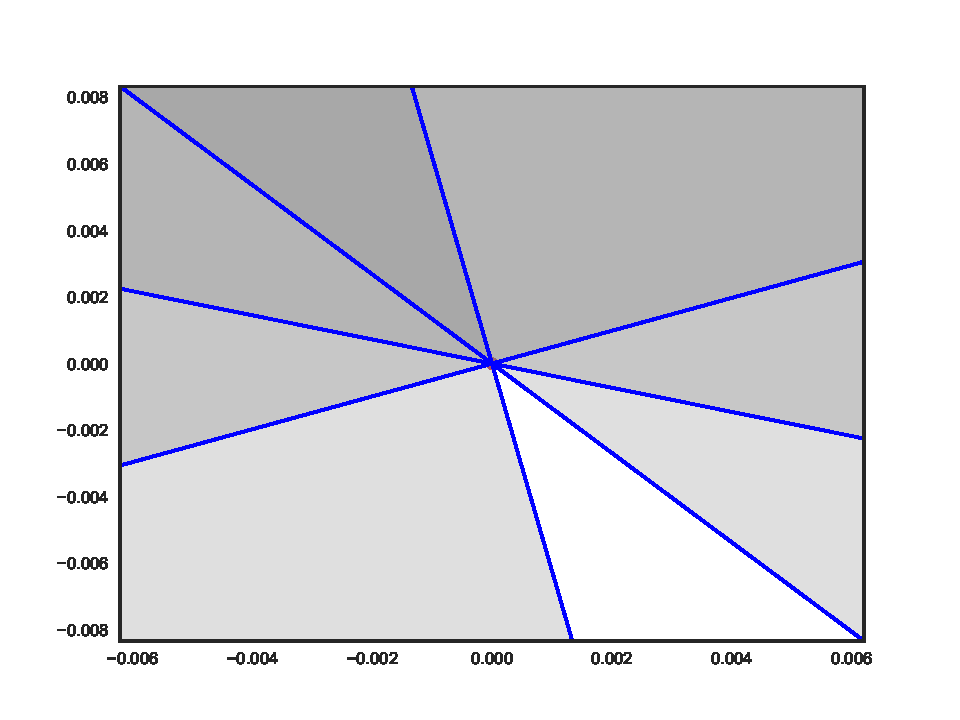
\includegraphics[width=\hsize]{img/toy/relu/conv2d_4-0.pdf}}
    %   \vskip1em
      \subcaptionbox{4th layer\label{fig:moonsReLU42}}{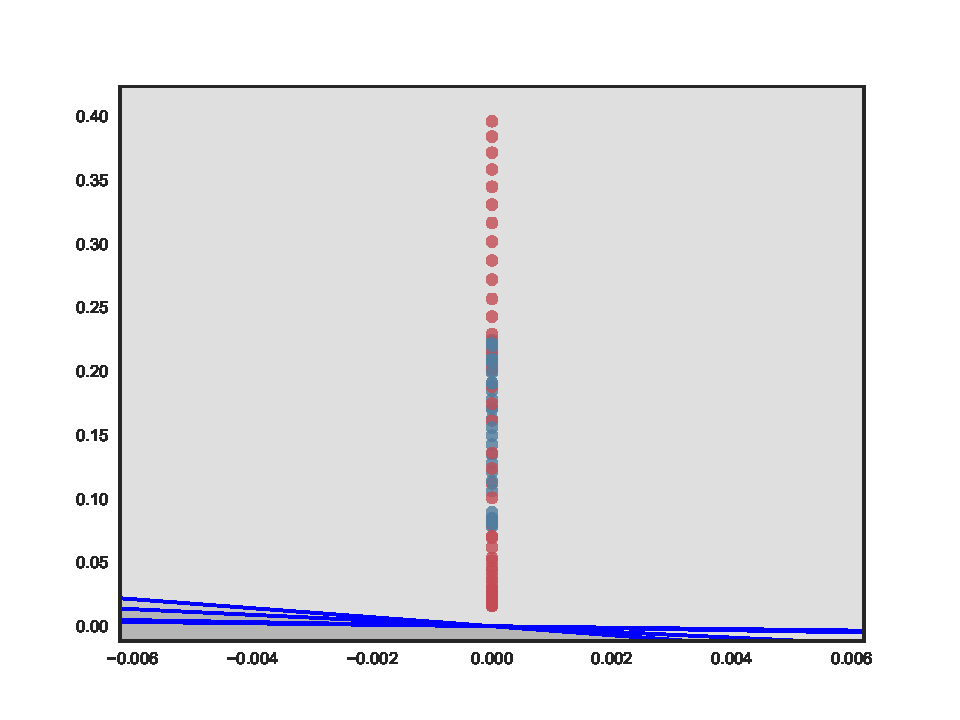
\includegraphics[width=\hsize]{img/toy/relu/conv2d_4-2.pdf}}
    }
    % \hskip1em
    \parbox{.195\textwidth}{%
      \subcaptionbox{25th layer\label{fig:moonsReLU251}}{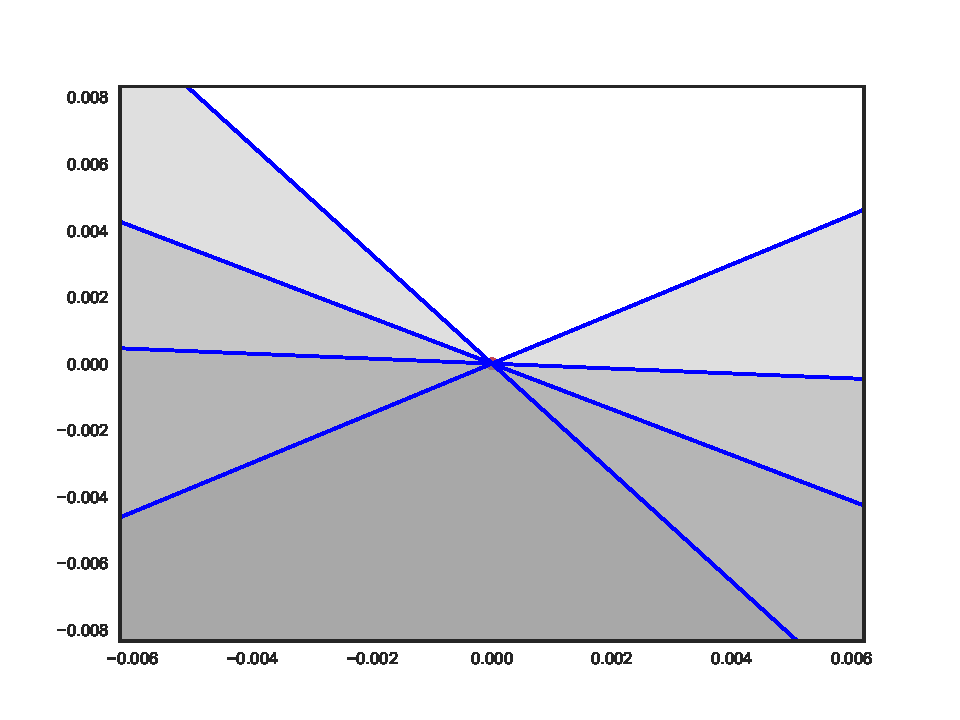
\includegraphics[width=\hsize]{img/toy/relu/conv2d_25-0.pdf}}
    %   \vskip1em
      \subcaptionbox{25th layer\label{fig:moonsReLU252}}{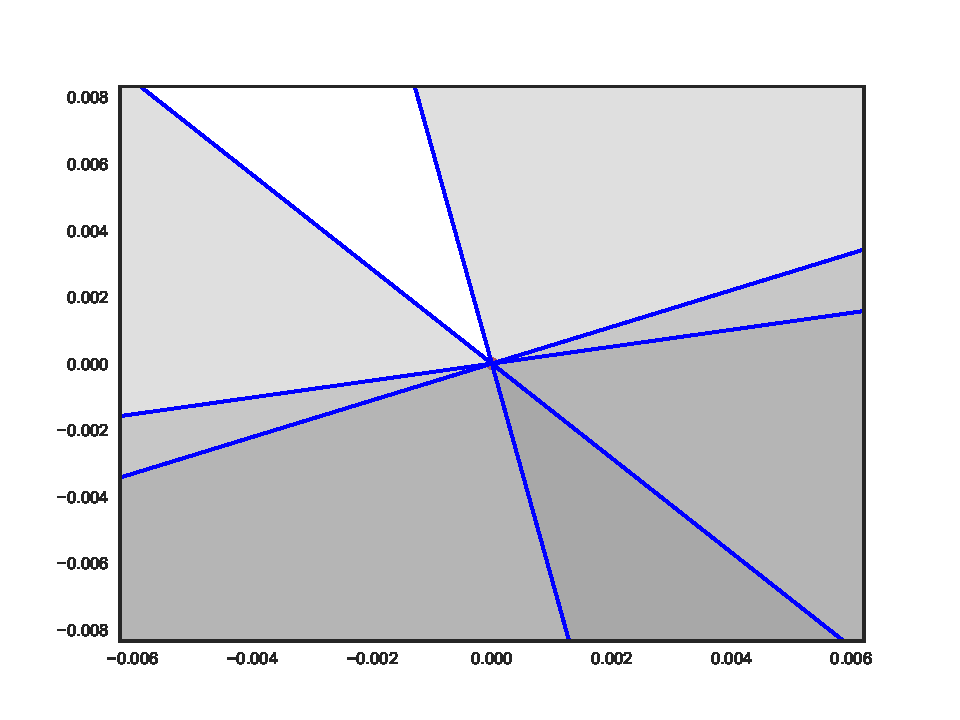
\includegraphics[width=\hsize]{img/toy/relu/conv2d_25-2.pdf}}
    }
    % \hskip1em
    \parbox{.195\textwidth}{%
      \subcaptionbox{Feature layer\label{fig:moonsReLUFeature1}}{\includegraphics[width=\hsize]{img/toy/relu/dense_1-0.pdf}}
    %   \vskip1em
      \subcaptionbox{Feature layer\label{fig:moonsReLUFeature2}}{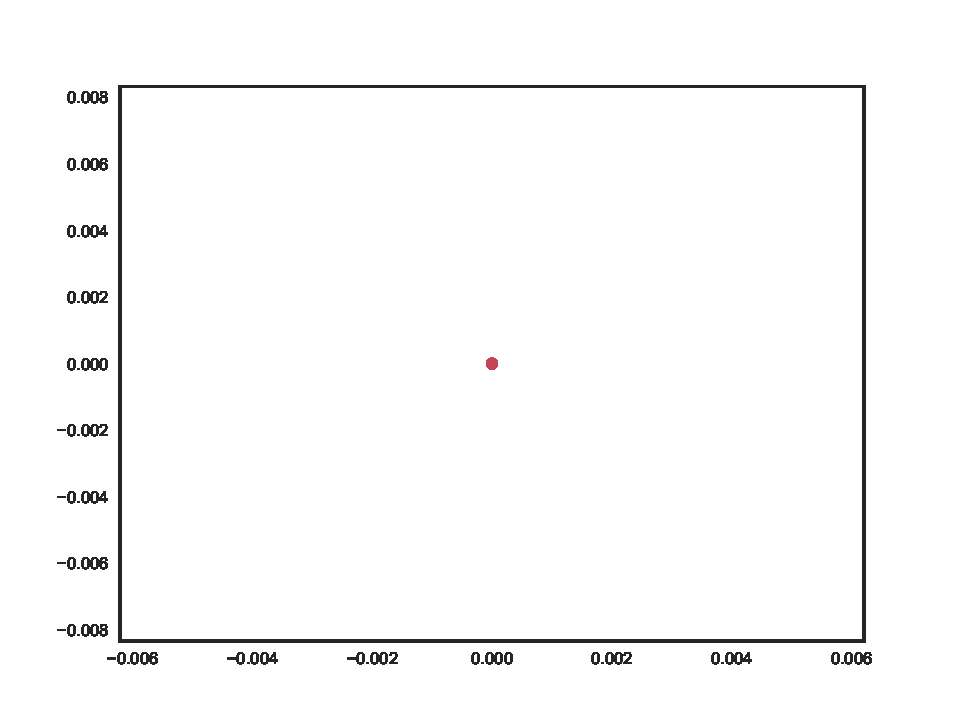
\includegraphics[width=\hsize]{img/toy/relu/dense_1-2.pdf}}
    }
    % \hskip1em
    \parbox{.195\textwidth}{%
      \subcaptionbox{Output\label{fig:moonsReLUOutput}}{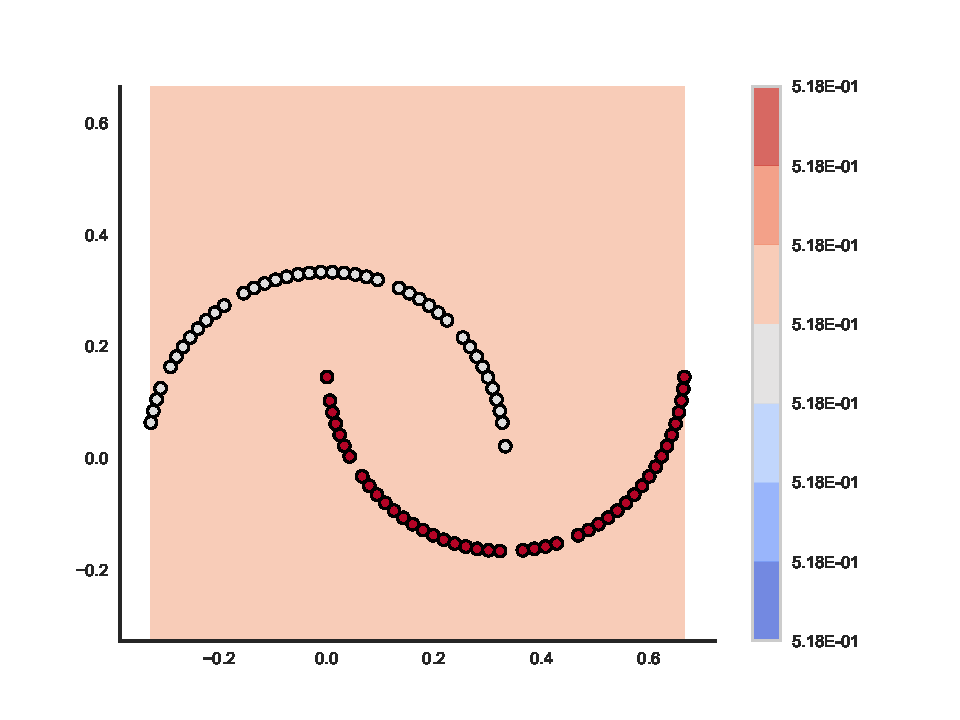
\includegraphics[width=\hsize]{img/toy/relu/output.pdf}}
    }
  }
  \caption{Data transformed across a 50x4 \ReLU classification network. Notice how the the dataset is progressively mapped to zero as it traverses the network. This renders the output layer unable to solve the problem.}
    \label{fig:moonsReLU}
\end{figure*}

\begin{figure*}
  \centering
  \parbox{\textwidth}{
    \parbox{.195\textwidth}{%
      \subcaptionbox{Input layer\label{fig:moonsReLUBNInput}}{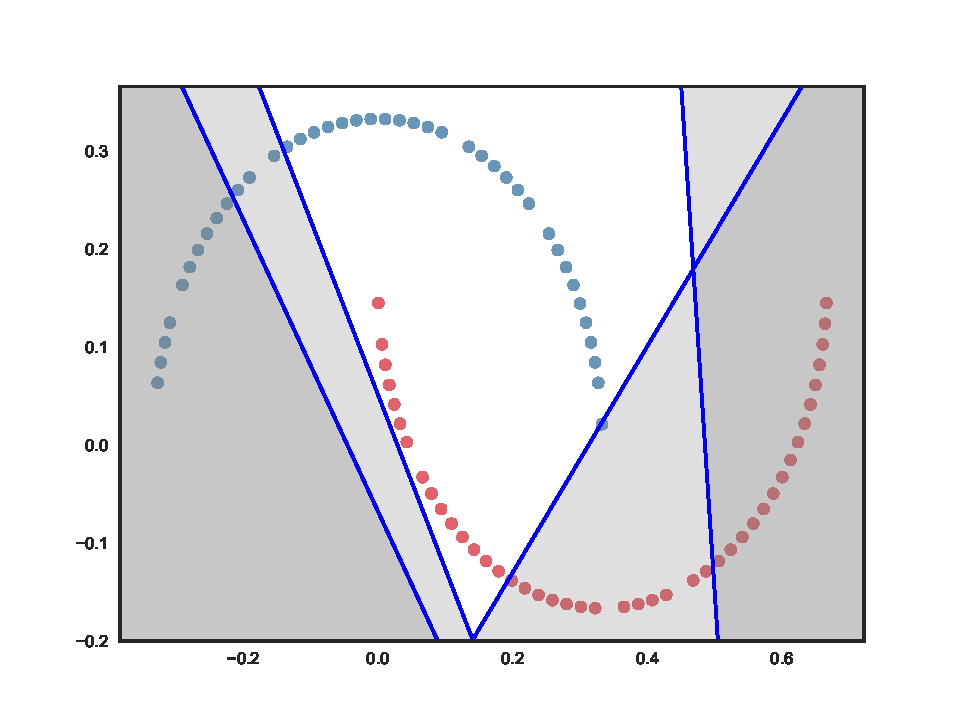
\includegraphics[width=\hsize]{img/toy/relu-bn/conv2d_1-0.pdf}}
    }
    % \hskip1em
    \parbox{.195\textwidth}{%
      \subcaptionbox{4th layer\label{fig:moonsReLUBN41}}{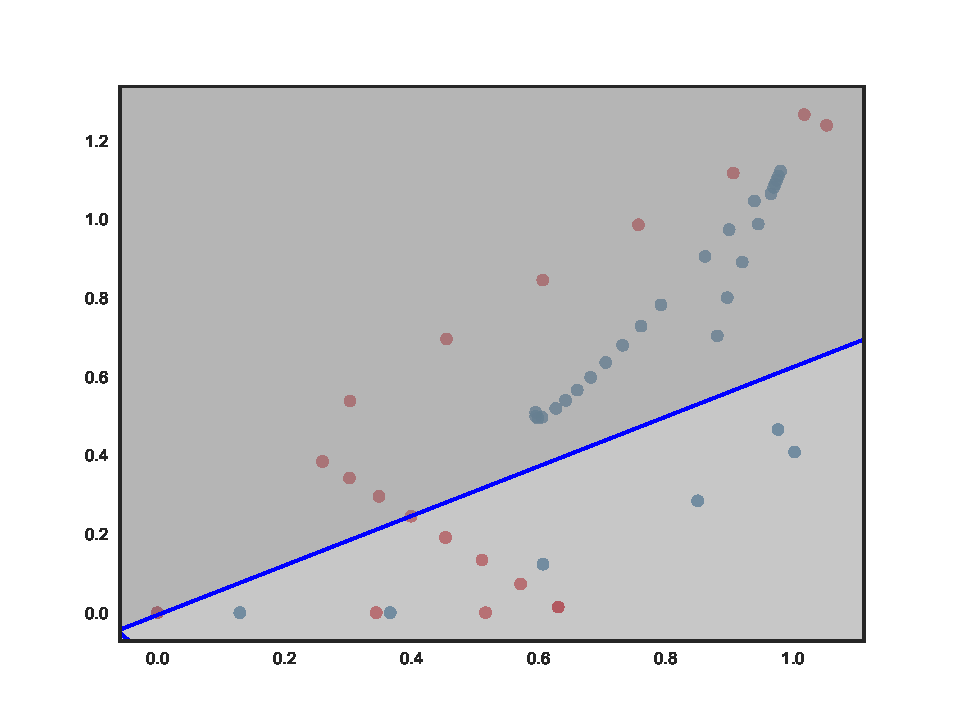
\includegraphics[width=\hsize]{img/toy/relu-bn/conv2d_4-0.pdf}}
    %   \vskip1em
      \subcaptionbox{4th layer\label{fig:moonsReLUBN42}}{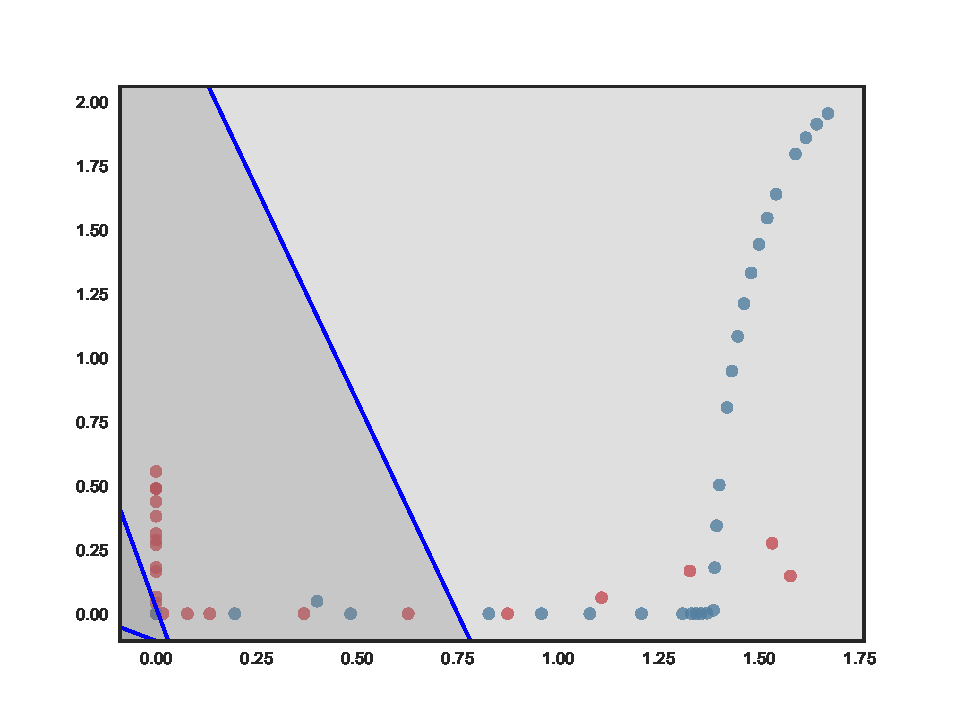
\includegraphics[width=\hsize]{img/toy/relu-bn/conv2d_4-2.pdf}}
    }
    % \hskip1em
    \parbox{.195\textwidth}{%
      \subcaptionbox{25th layer\label{fig:moonsReLUBN251}}{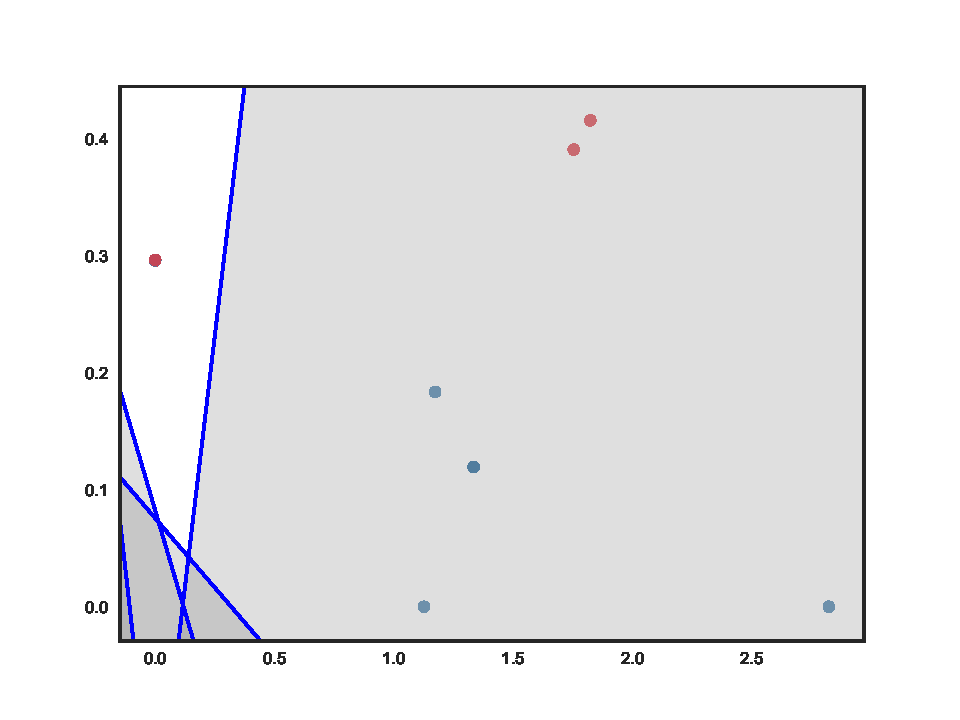
\includegraphics[width=\hsize]{img/toy/relu-bn/conv2d_25-0.pdf}}
    %   \vskip1em
      \subcaptionbox{25th layer\label{fig:moonsReLUBN252}}{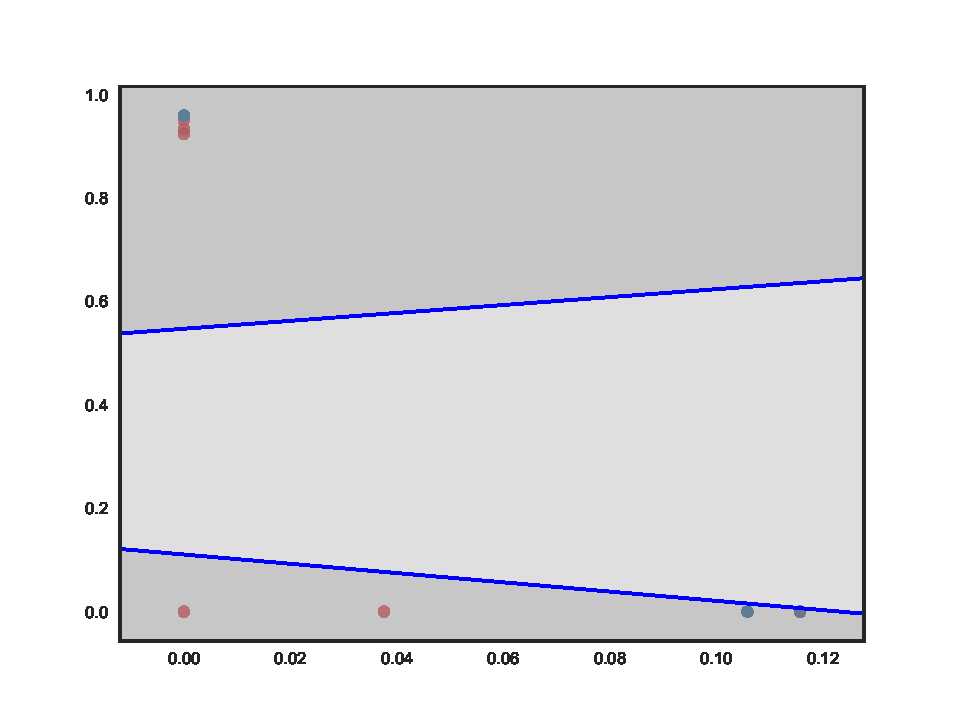
\includegraphics[width=\hsize]{img/toy/relu-bn/conv2d_25-2.pdf}} 
    }
    % \hskip1em
    \parbox{.195\textwidth}{%
      \subcaptionbox{Feature layer\label{fig:moonsReLUBNFeature1}}{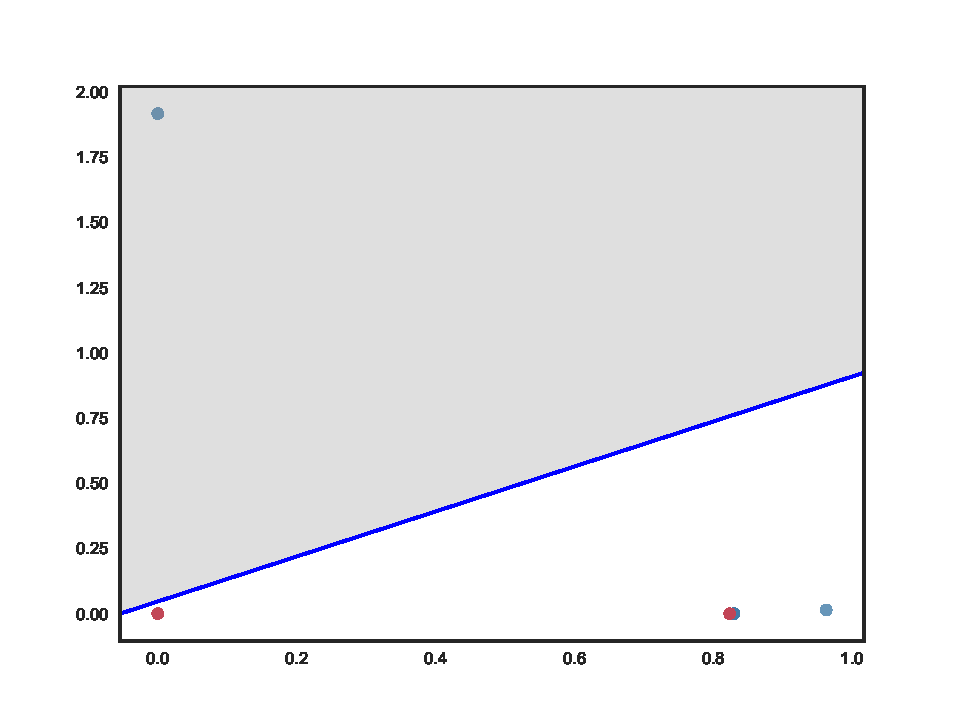
\includegraphics[width=\hsize]{img/toy/relu-bn/dense_1-0.pdf}}
    %   \vskip1em
      \subcaptionbox{Feature layer\label{fig:moonsReLUBNFeature2}}{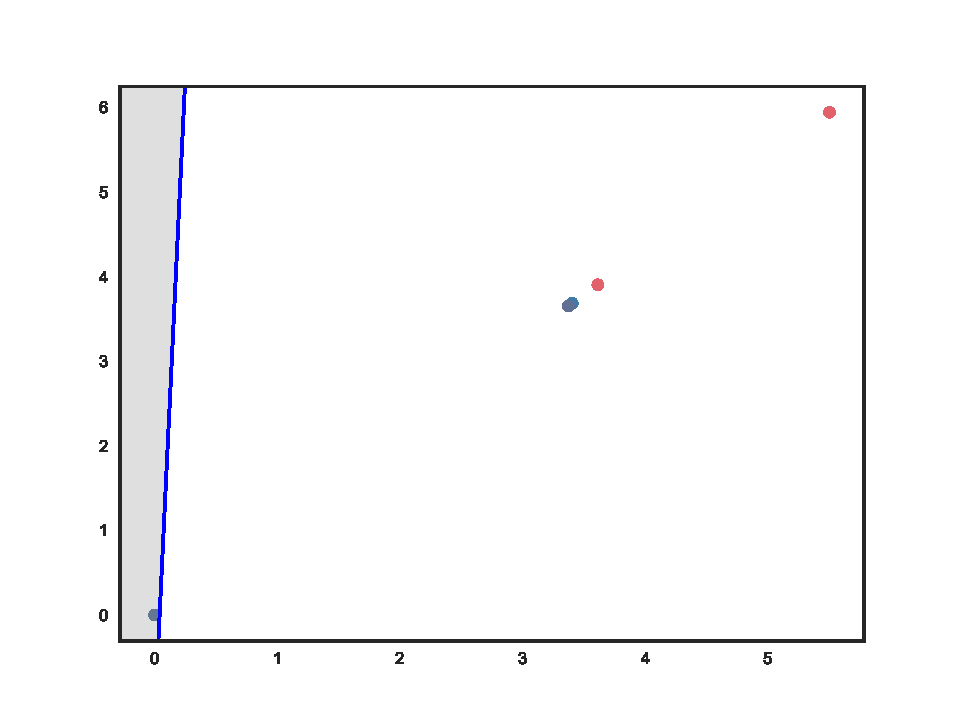
\includegraphics[width=\hsize]{img/toy/relu-bn/dense_1-2.pdf}} 
    }
    % \hskip1em
    \parbox{.195\textwidth}{%
      \subcaptionbox{Output\label{fig:moonsReLUBNOutput}}{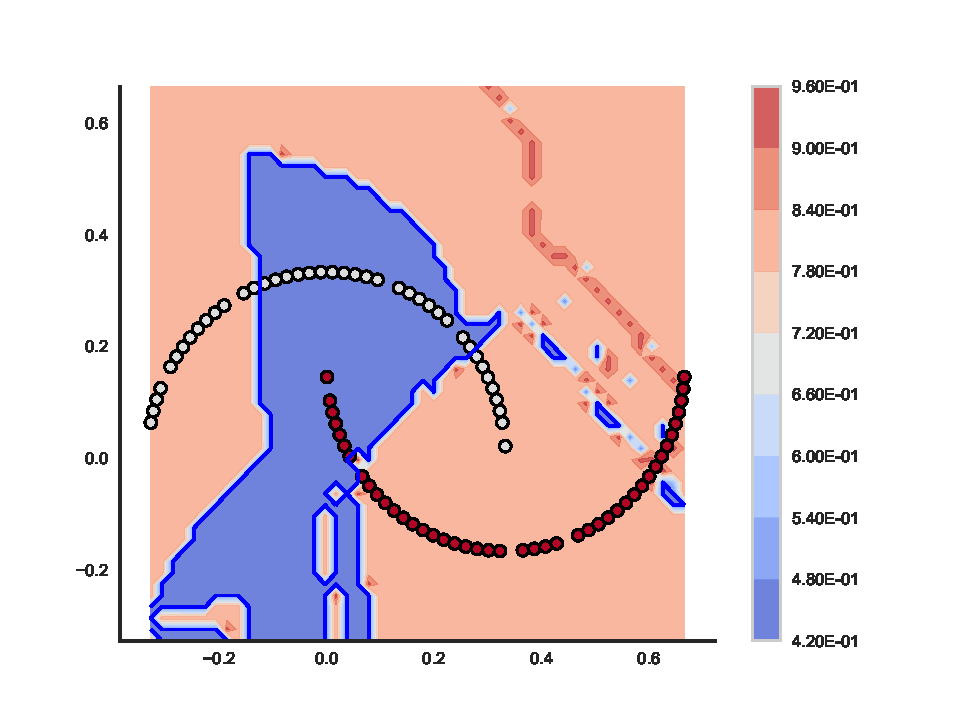
\includegraphics[width=\hsize]{img/toy/relu-bn/output.pdf}}
    }
  }
  \caption{Data transformed across a 50x4 \ReLUBN network. As the gradient cannot be backpropagated across the \ReLU, the non-trivial activations generated by Batch Normalization are based on the arbitrary position of the hyperplanes after intialization rather the actual topology of the dataset. This results in \emph{topological mixing} of the dataset across the layers, resulting in mapping the entire dataset to four points in the feature layer. Therefore, the representational capability of the network is hindered to such extent that the resulting output, although non-trivial, is totally arbitrary.}
    \label{fig:moonsReLUBN}
\end{figure*}





\begin{figure*}
  \centering
  \parbox{\textwidth}{
    \parbox{.195\textwidth}{%
      \subcaptionbox{Input layer\label{fig:moonsLayerwiseInput}}{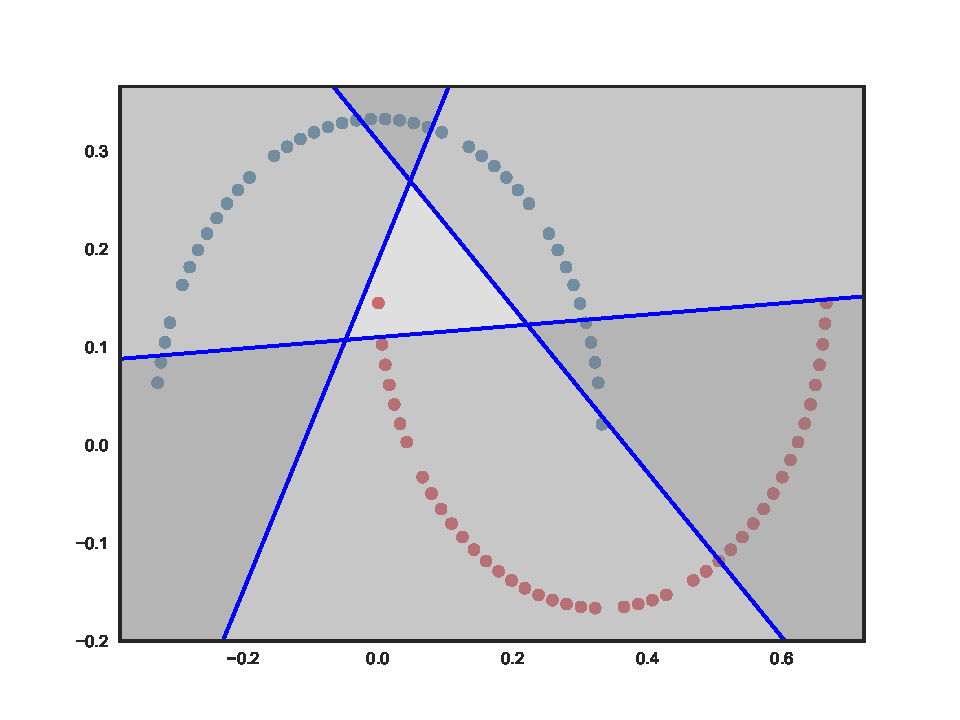
\includegraphics[width=\hsize]{img/toy/layerwise/conv2d_1-0.pdf}}
    }
    % \hskip1em
    \parbox{.195\textwidth}{%
      \subcaptionbox{4th layer\label{fig:moonsLayerwise41}}{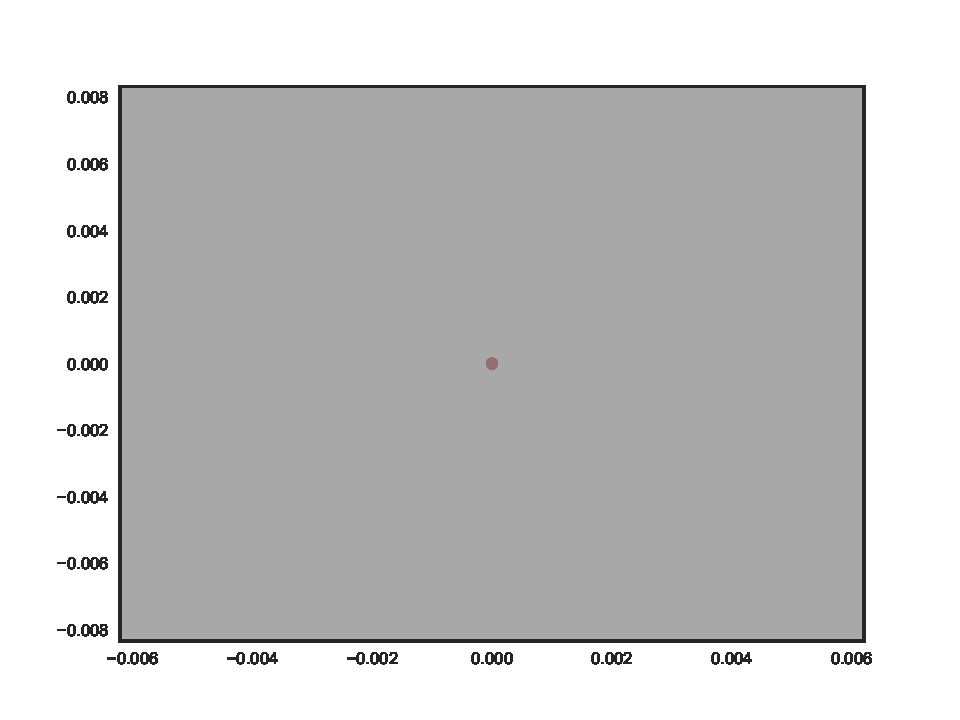
\includegraphics[width=\hsize]{img/toy/layerwise/conv2d_4-0.pdf}}
    %   \vskip1em
      \subcaptionbox{4th layer\label{fig:moonsLayerwise42}}{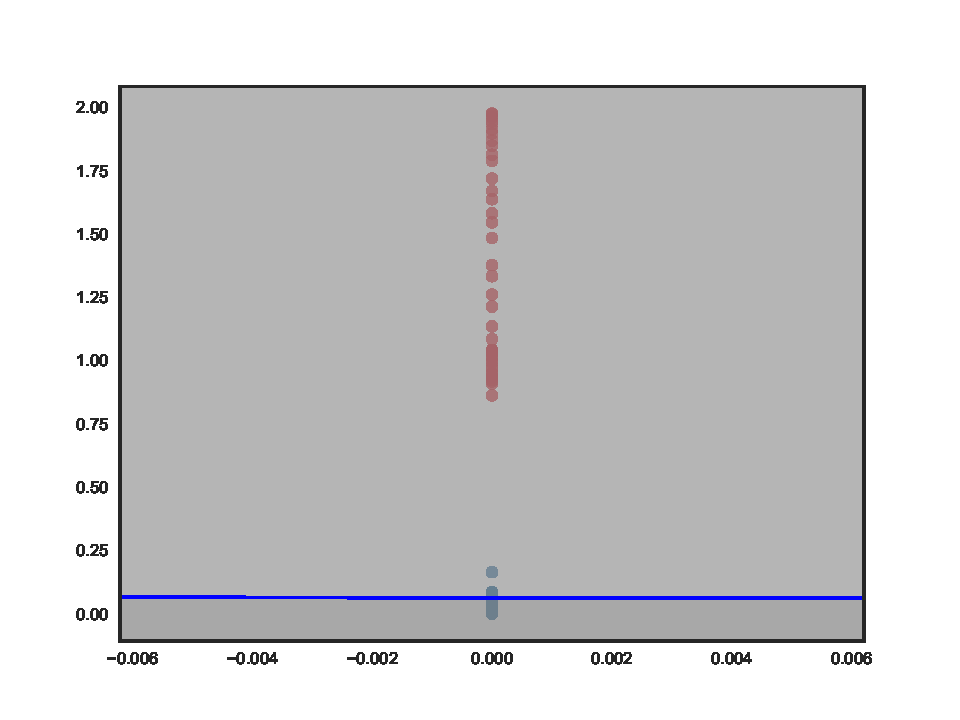
\includegraphics[width=\hsize]{img/toy/layerwise/conv2d_4-2.pdf}} 
    }
    % \hskip1em
    \parbox{.195\textwidth}{%
      \subcaptionbox{25th layer\label{fig:moonsLayerwise251}}{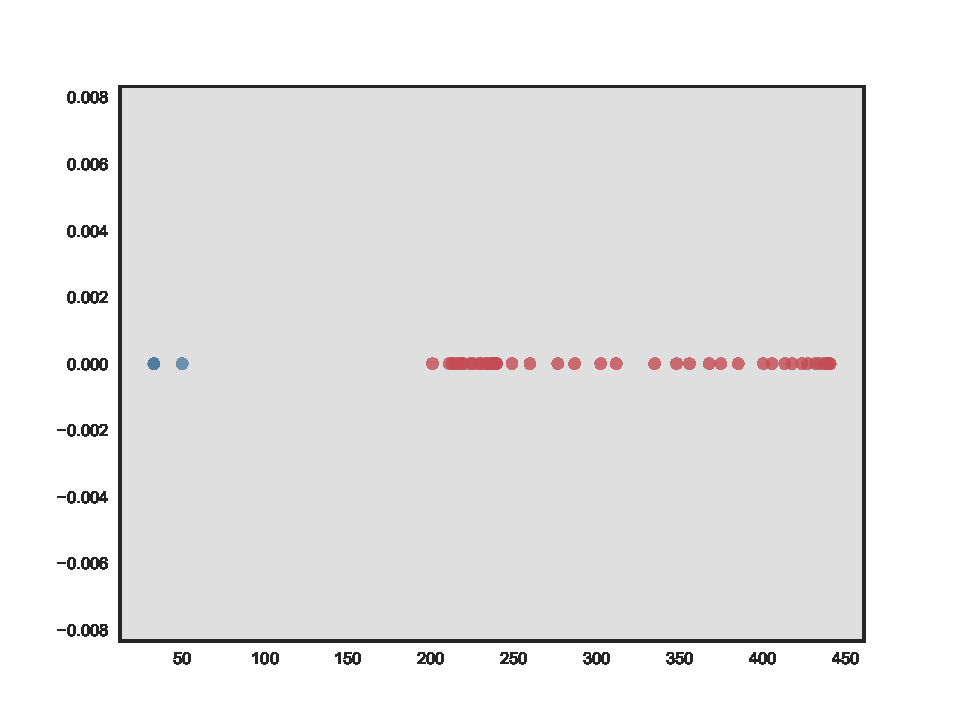
\includegraphics[width=\hsize]{img/toy/layerwise/conv2d_25-0.pdf}}
    %   \vskip1em
      \subcaptionbox{25th layer\label{fig:moonsLayerwise251}}{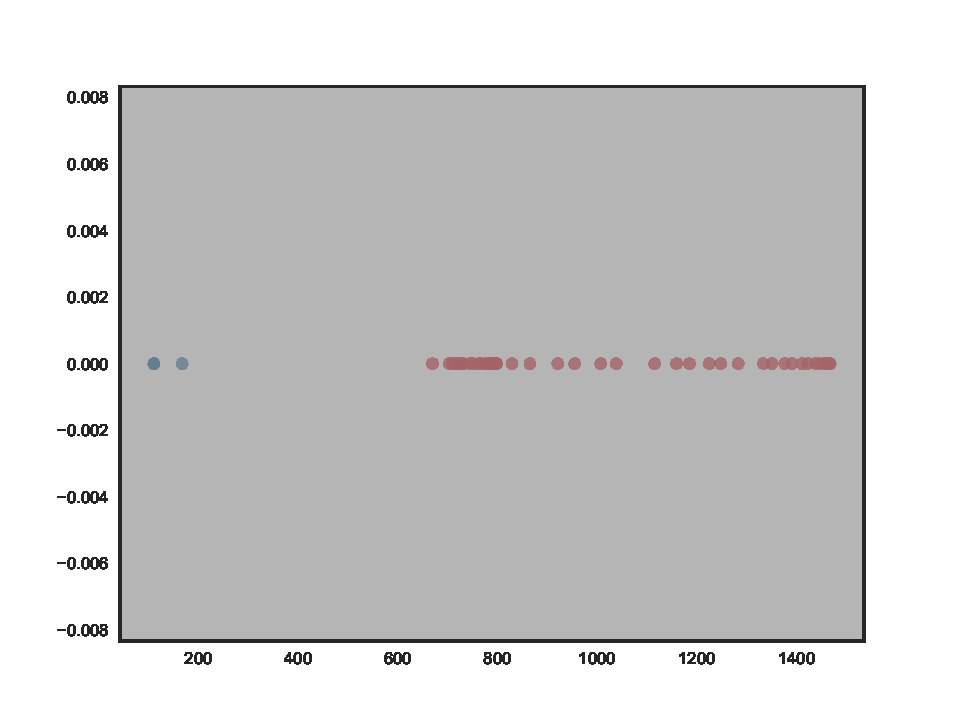
\includegraphics[width=\hsize]{img/toy/layerwise/conv2d_25-2.pdf}} 
    }
    % \hskip1em
    \parbox{.195\textwidth}{%
      \subcaptionbox{Feature layer\label{fig:moonsLayerwiseFeature1}}{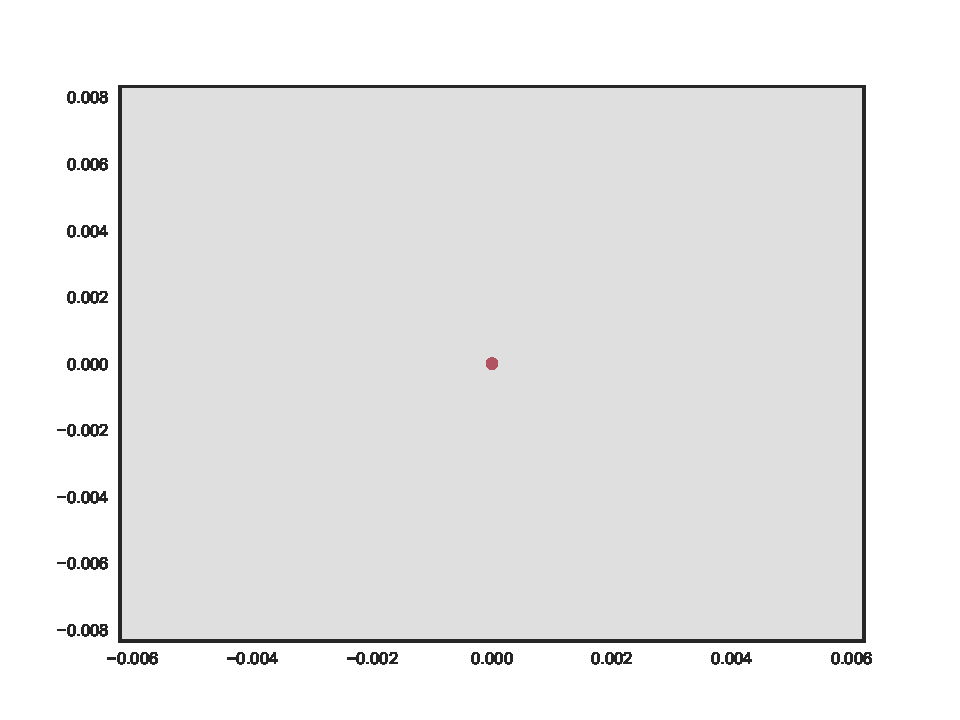
\includegraphics[width=\hsize]{img/toy/layerwise/dense_1-0.pdf}}
    %   \vskip1em
      \subcaptionbox{Feature layer\label{fig:moonsLayerwiseFeature2}}{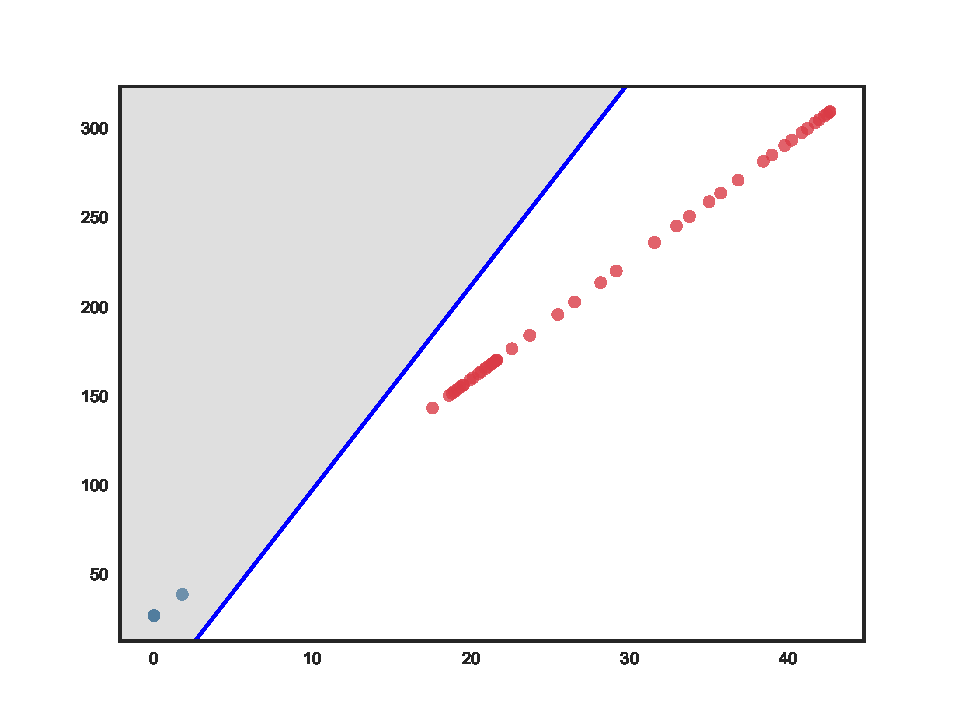
\includegraphics[width=\hsize]{img/toy/layerwise/dense_1-2.pdf}} 
    }
    % \hskip1em
    \parbox{.195\textwidth}{%
      \subcaptionbox{Output\label{fig:moonsLayerwiseOutput}}{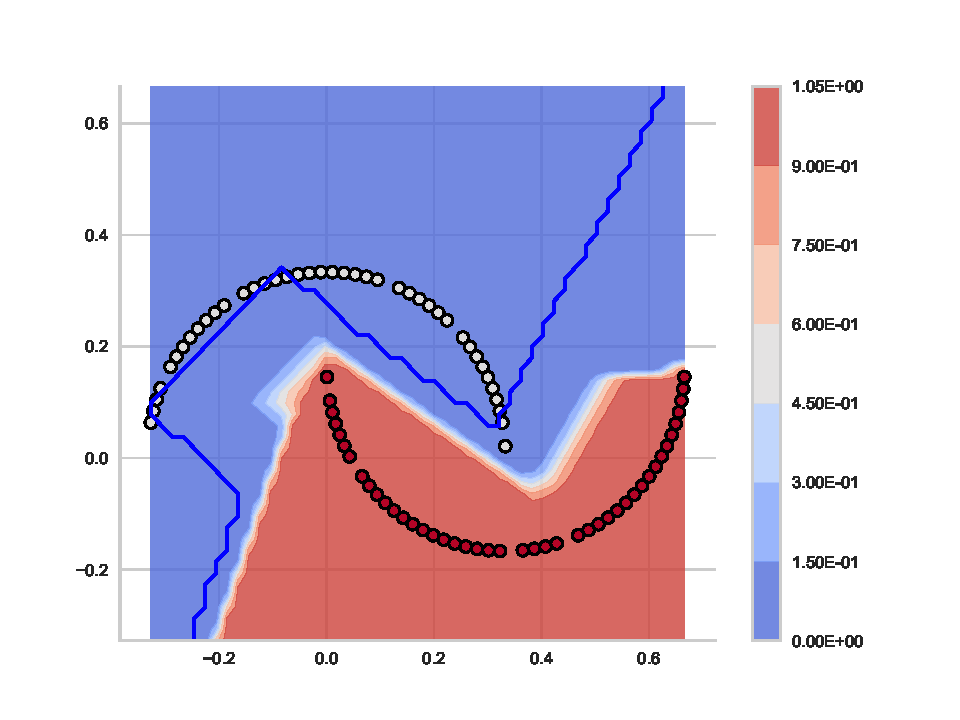
\includegraphics[width=\hsize]{img/toy/layerwise/output.pdf}}
    }
  }
    \caption{\SepLayer}
    \label{fig:moonsLayerwise}
\end{figure*}




\begin{figure*}
  \centering
     % Unitwise
  \parbox{\textwidth}{
    \parbox{.195\textwidth}{%
      \subcaptionbox{Input layer\label{fig:moonsUnitwiseInput}}{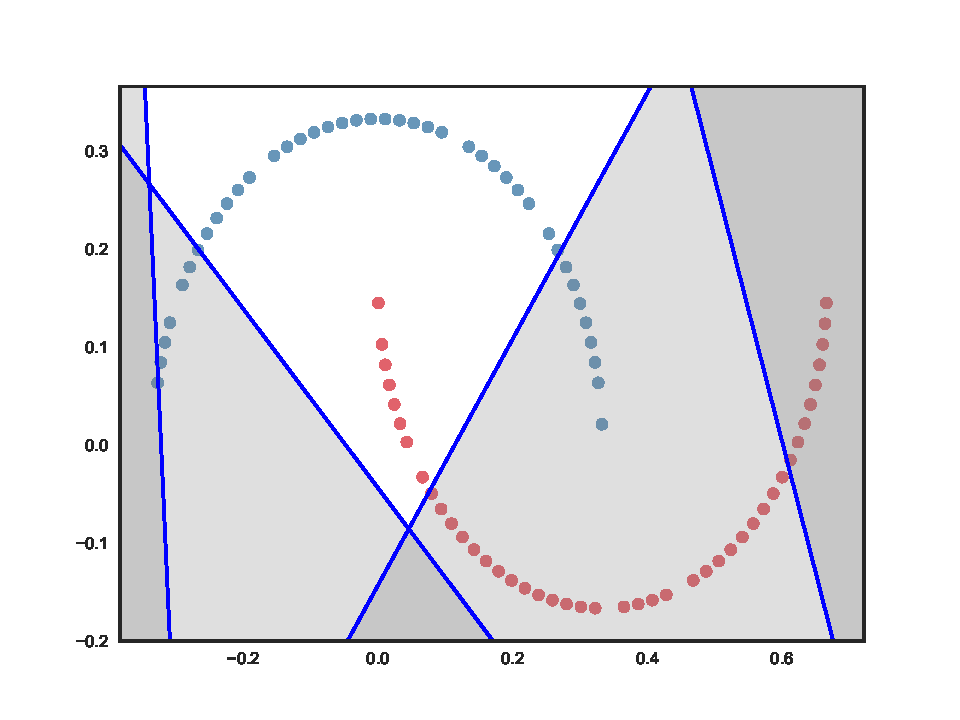
\includegraphics[width=\hsize]{img/toy/unitwise/conv2d_1-0.pdf}}
    }
    % \hskip1em
    \parbox{.195\textwidth}{%
      \subcaptionbox{4th layer\label{fig:moonsUnitwise41}}{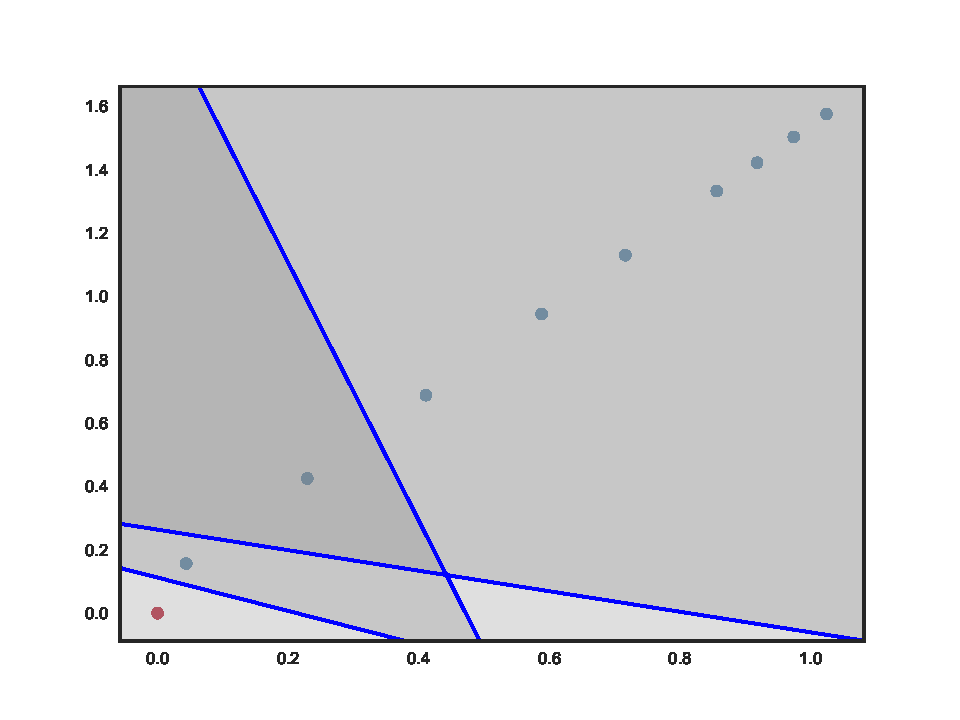
\includegraphics[width=\hsize]{img/toy/unitwise/conv2d_4-0.pdf}}
    %   \vskip1em
      \subcaptionbox{4th layer\label{fig:moonsUnitwise42}}{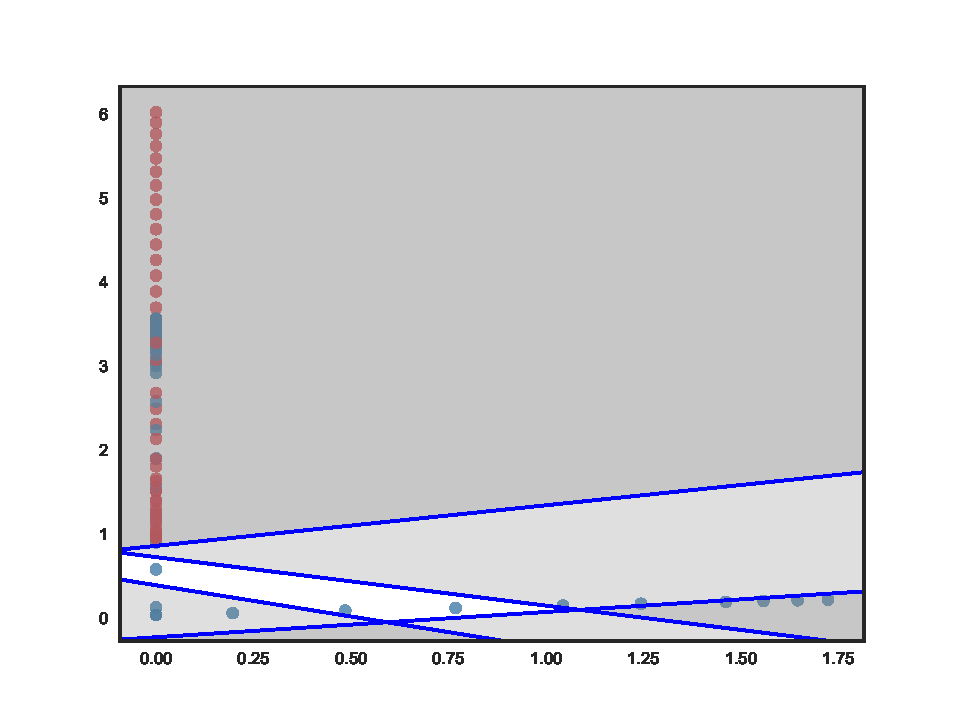
\includegraphics[width=\hsize]{img/toy/unitwise/conv2d_4-2.pdf}}
    }
    % \hskip1em
    \parbox{.195\textwidth}{%
      \subcaptionbox{25th layer\label{fig:moonsUnitwise251}}{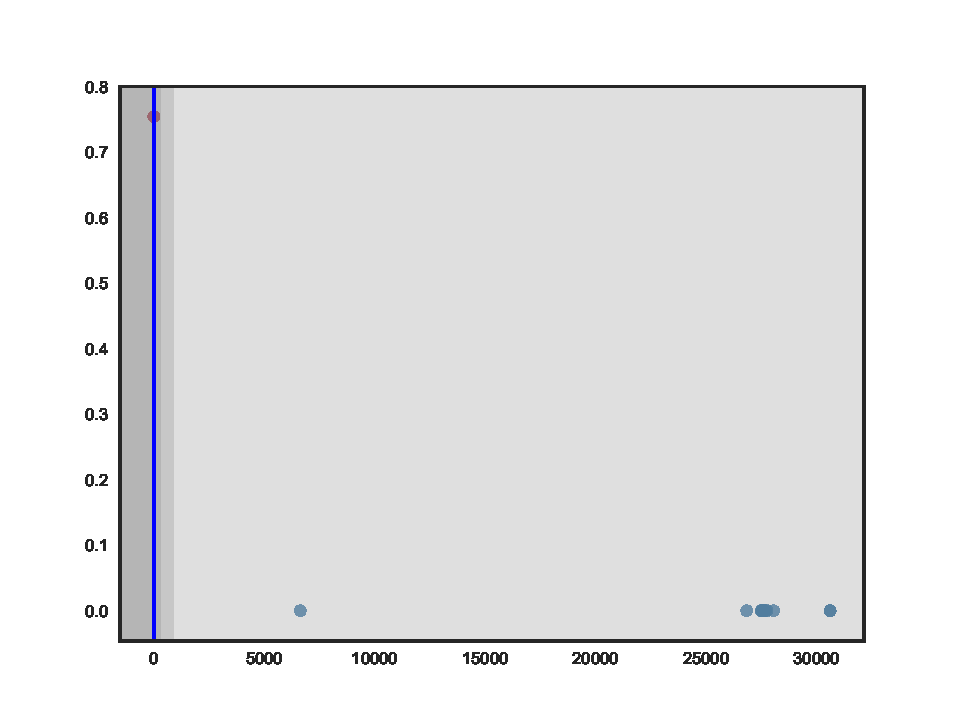
\includegraphics[width=\hsize]{img/toy/unitwise/conv2d_25-0.pdf}}
    %   \vskip1em
      \subcaptionbox{25th layer\label{fig:moonsUnitwise252}}{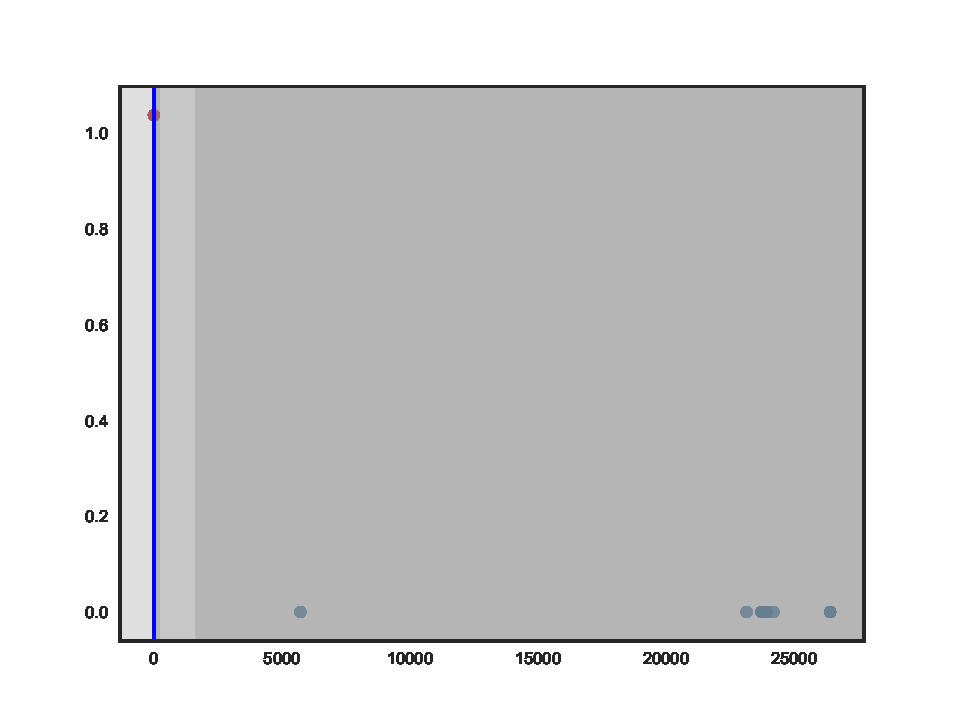
\includegraphics[width=\hsize]{img/toy/unitwise/conv2d_25-2.pdf}}
    }
    % \hskip1em
    \parbox{.195\textwidth}{%
      \subcaptionbox{Feature layer\label{fig:moonsUnitwiseFeature1}}{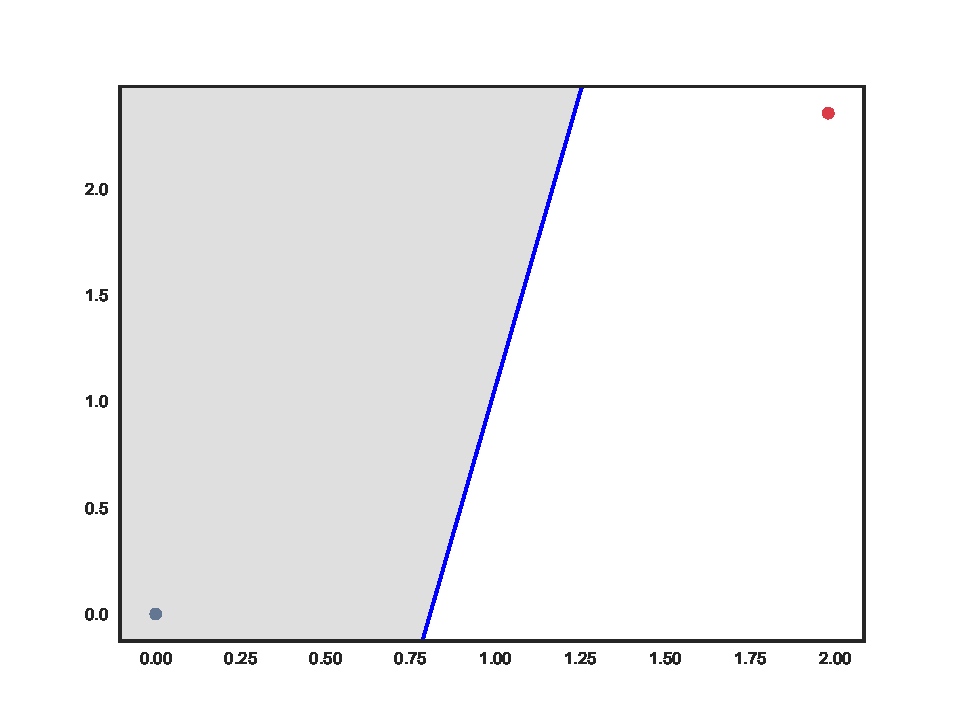
\includegraphics[width=\hsize]{img/toy/unitwise/dense_1-0.pdf}}
    %   \vskip1em
      \subcaptionbox{Feature layer\label{fig:moonsUnitwiseFeature2}}{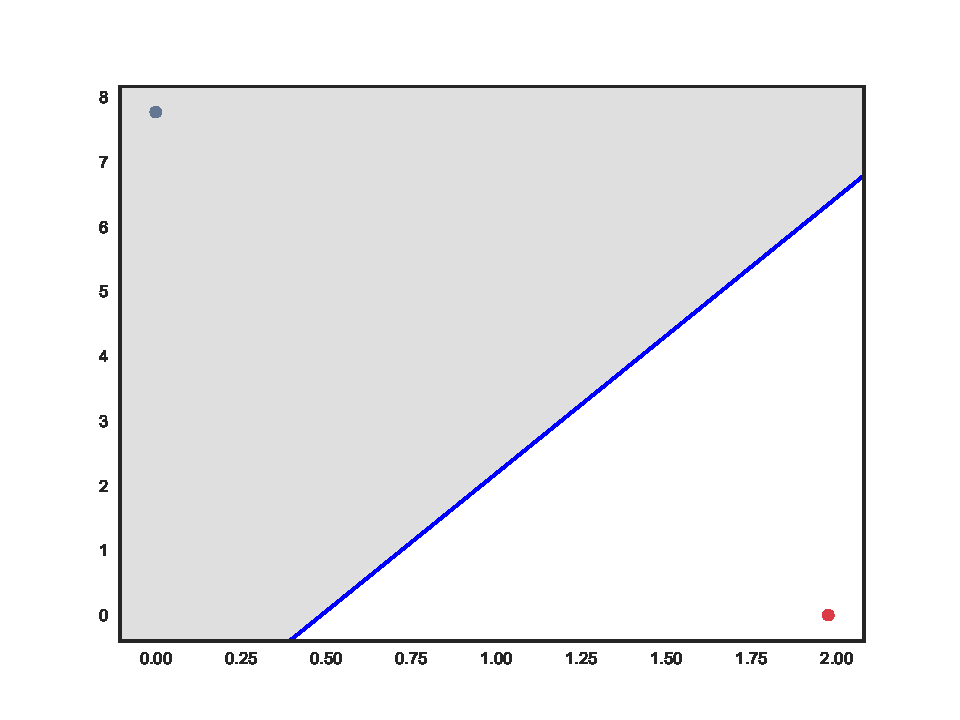
\includegraphics[width=\hsize]{img/toy/unitwise/dense_1-2.pdf}}
    }
    % \hskip1em
    \parbox{.195\textwidth}{%
      \subcaptionbox{Output\label{fig:moonsUnitwiseOutput}}{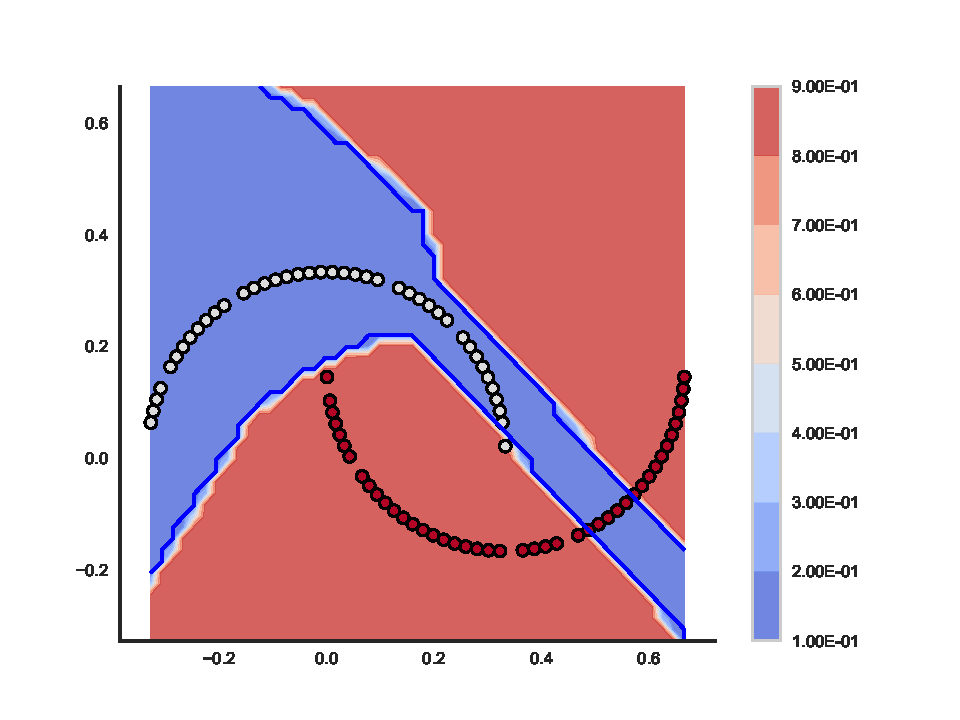
\includegraphics[width=\hsize]{img/toy/unitwise/output.pdf}}
    }
  }
  \caption{\SepUnit}
    \label{fig:moonsUnitwise}
\end{figure*}



\begin{figure*}
  \centering
  %Pointwise
  \parbox{\textwidth}{
    \parbox{.195\textwidth}{%
      \subcaptionbox{Input layer\label{fig:moonsPointwiseInput}}{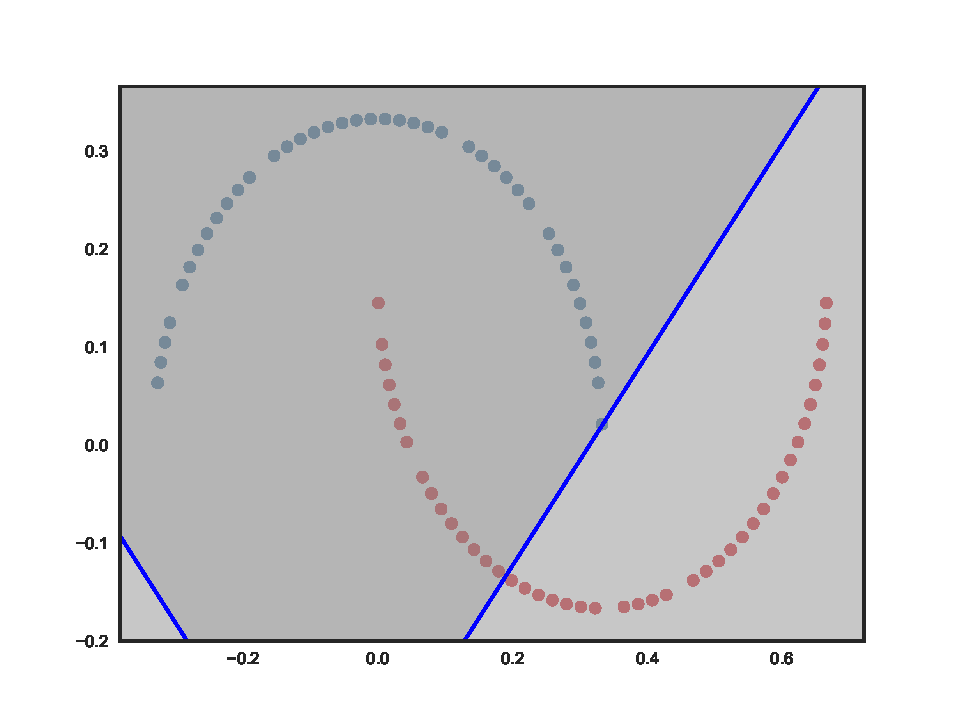
\includegraphics[width=\hsize]{img/toy/pointwise/conv2d_1-0.pdf}}
    }
    % \hskip1em
    \parbox{.195\textwidth}{%
      \subcaptionbox{4th layer\label{fig:moonsPointwise41}}{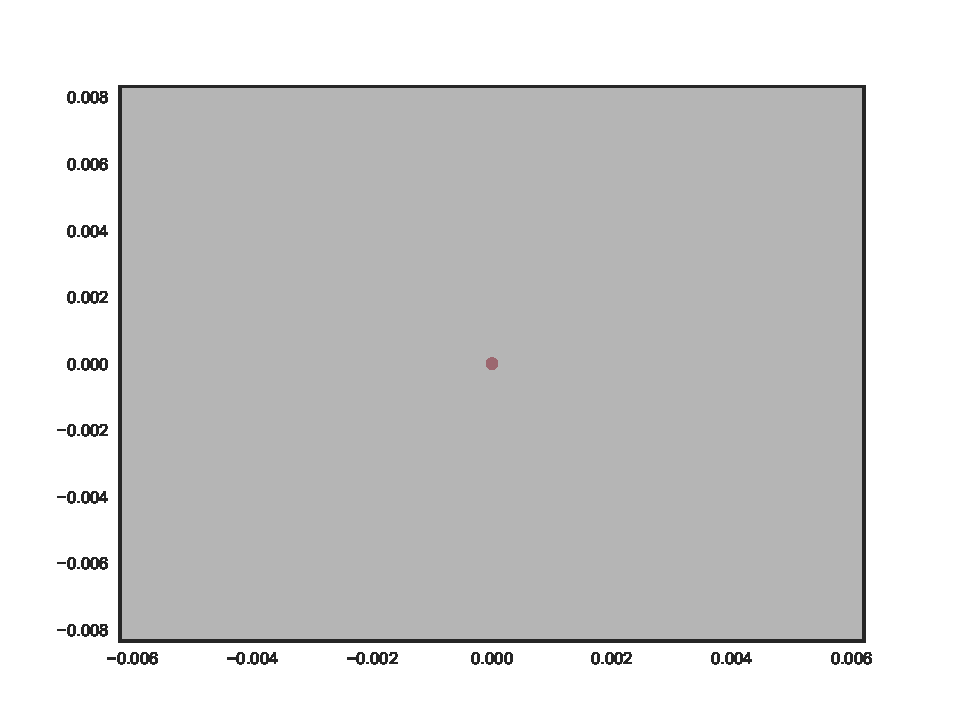
\includegraphics[width=\hsize]{img/toy/pointwise/conv2d_4-0.pdf}}
    %   \vskip1em
      \subcaptionbox{4th layer\label{fig:moonsPointwise42}}{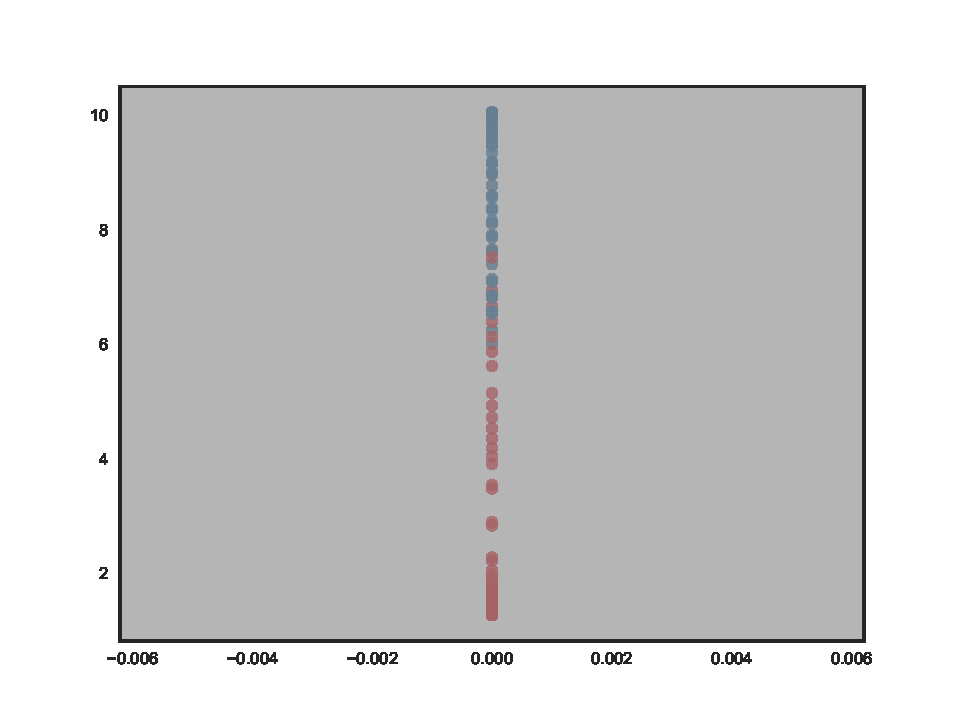
\includegraphics[width=\hsize]{img/toy/pointwise/conv2d_4-2.pdf}} 
    }
    % \hskip1em
    \parbox{.195\textwidth}{%
      \subcaptionbox{25th layer\label{fig:moonsPointwise251}}{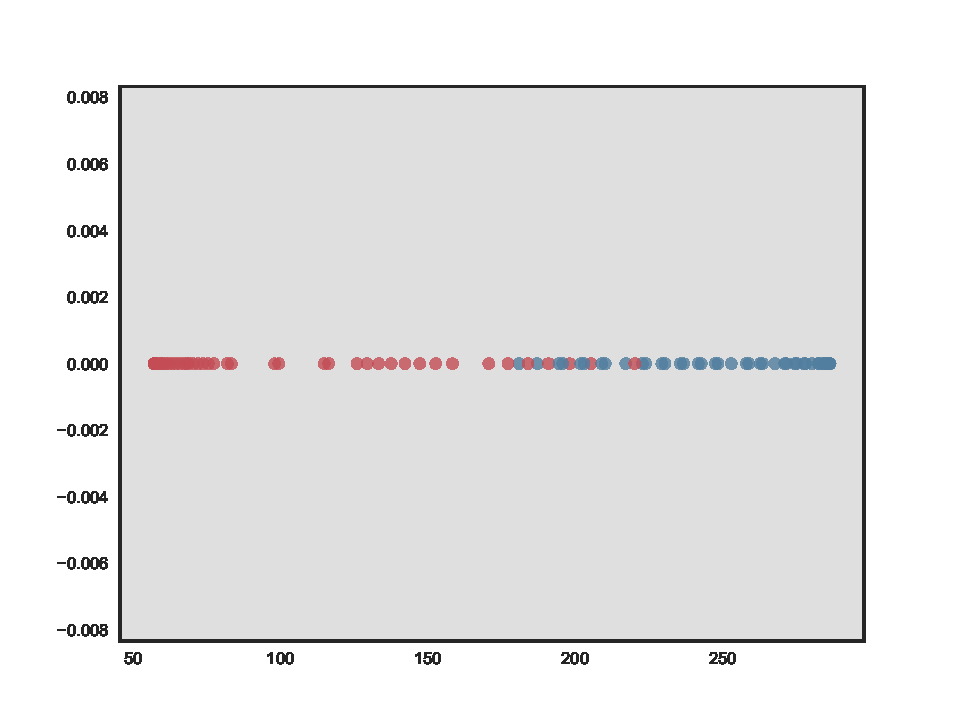
\includegraphics[width=\hsize]{img/toy/pointwise/conv2d_25-0.pdf}}
    %   \vskip1em
      \subcaptionbox{25th layer\label{fig:moonsPointwise252}}{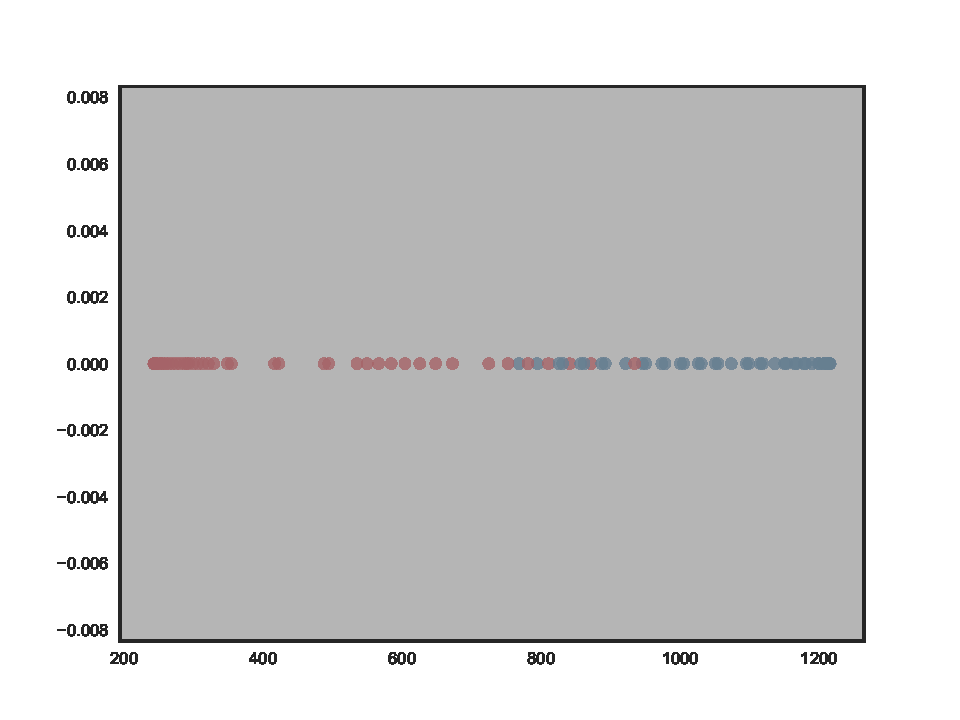
\includegraphics[width=\hsize]{img/toy/pointwise/conv2d_25-2.pdf}} 
    }
    % \hskip1em
    \parbox{.195\textwidth}{%
      \subcaptionbox{\label{fig:moonsPointwiseFeature1}}{\includegraphics[width=\hsize]{img/toy/pointwise/dense_1-0.pdf}}
    %   \vskip1em
      \subcaptionbox{\label{fig:moonsPointwiseFeature2}}{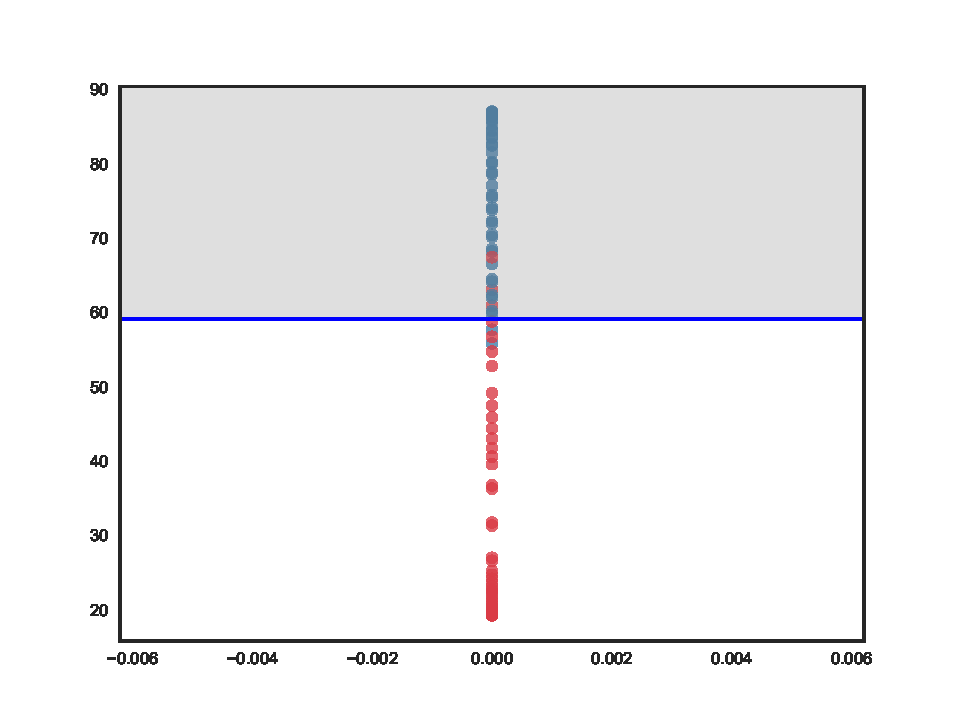
\includegraphics[width=\hsize]{img/toy/pointwise/dense_1-2.pdf}} 
    }
    % \hskip1em
    \parbox{.195\textwidth}{%
      \subcaptionbox{Output\label{fig:moonsPointwiseOutput}}{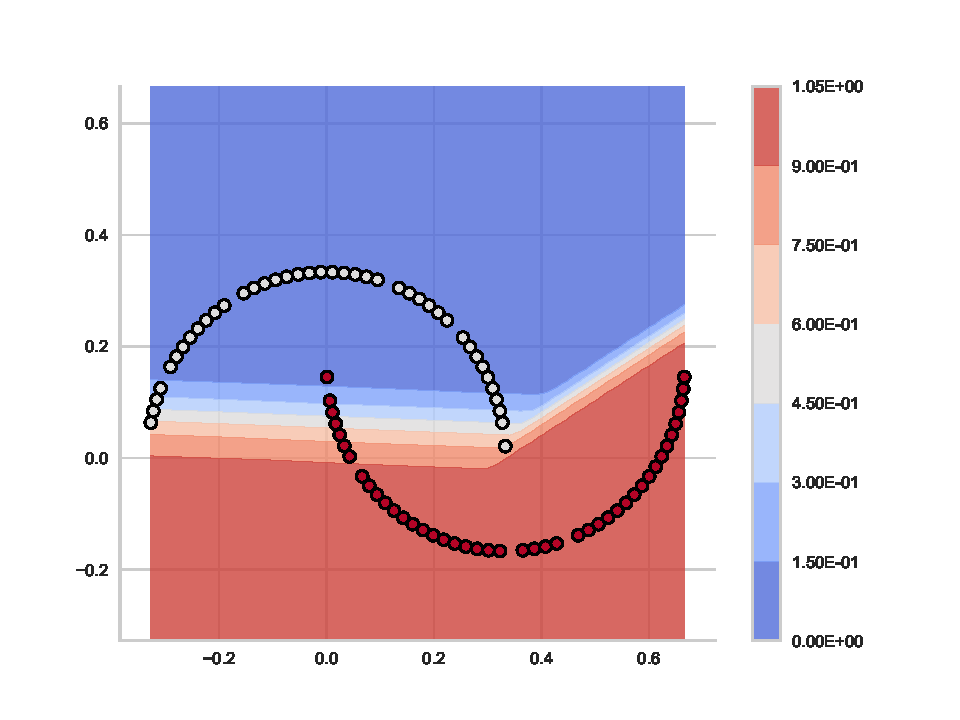
\includegraphics[width=\hsize]{img/toy/pointwise/output.pdf}}
    }
  }
  \caption{\SepPoint}
    \label{fig:moonsPointwise}
\end{figure*}


\begin{figure*}
  \centering
   \parbox{\textwidth}{
    \parbox{.195\textwidth}{%
      \subcaptionbox{Input layer\label{fig:moonsUnitpointwiseInput}}{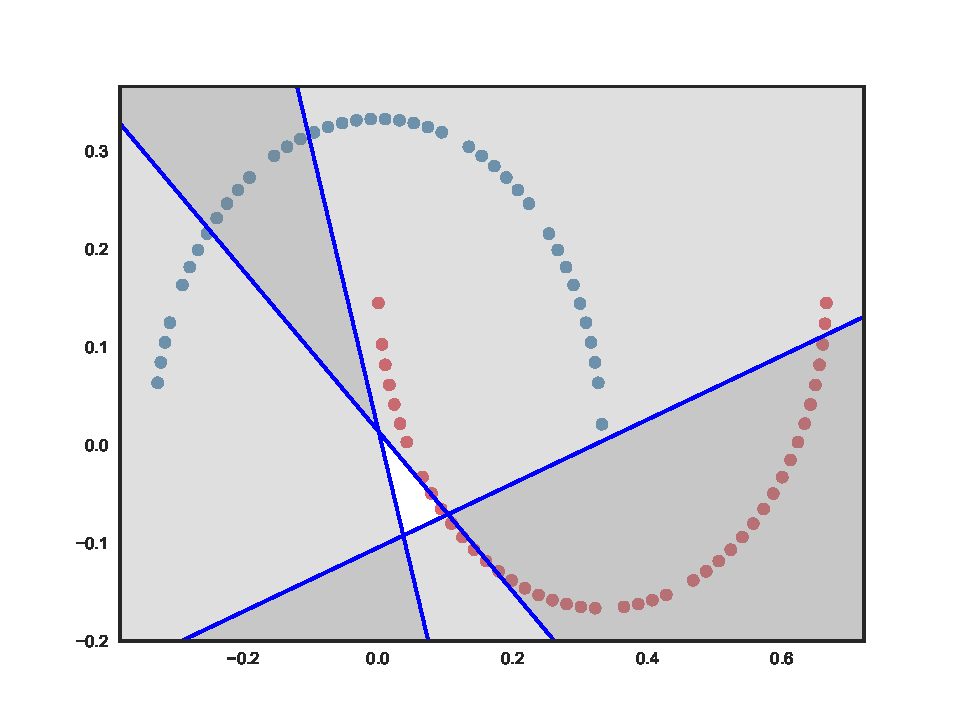
\includegraphics[width=\hsize]{img/toy/unitpointwise/conv2d_1-0.pdf}}
    }
    % \hskip1em
    \parbox{.195\textwidth}{%
      \subcaptionbox{4th layer\label{fig:moonsUnitpointwise41}}{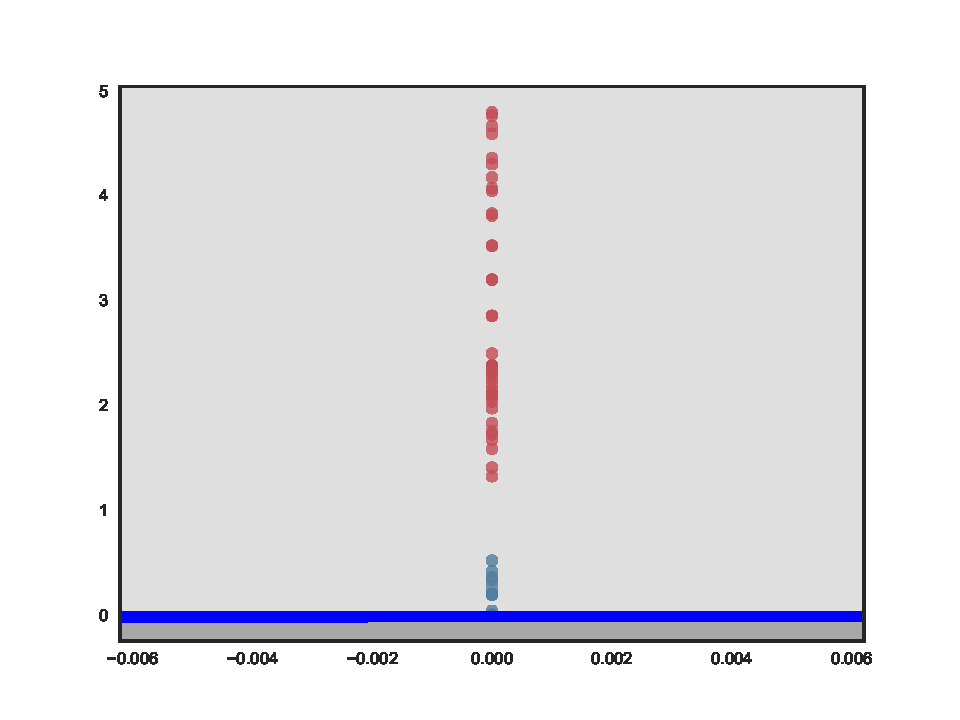
\includegraphics[width=\hsize]{img/toy/unitpointwise/conv2d_4-0.pdf}}
    %   \vskip1em
      \subcaptionbox{4th layer\label{fig:moonsUnitpointwise42}}{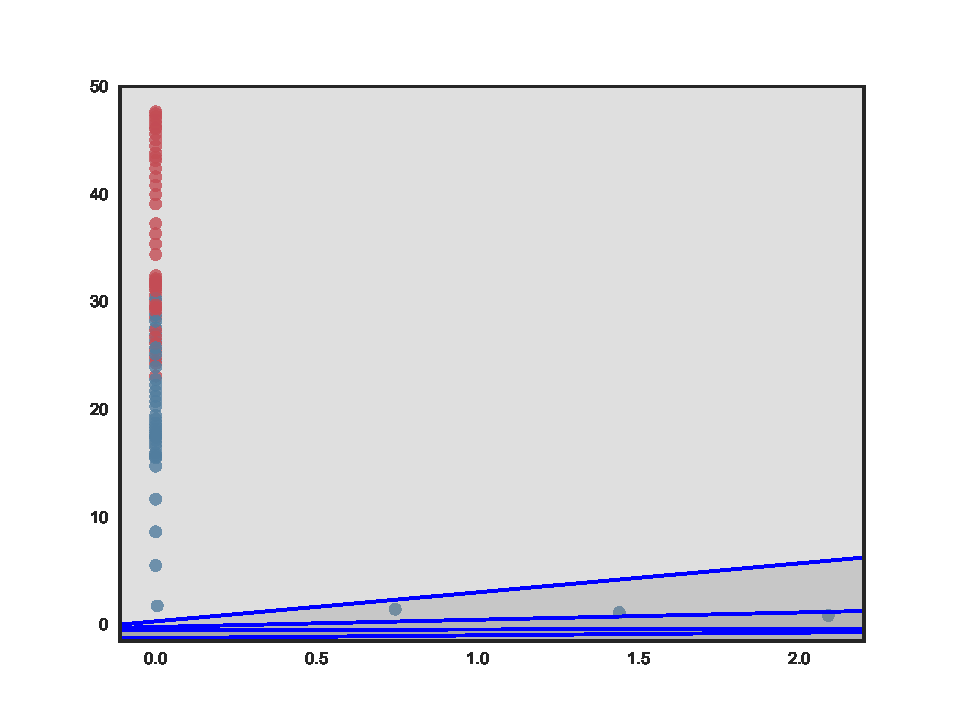
\includegraphics[width=\hsize]{img/toy/unitpointwise/conv2d_4-2.pdf}} 
    }
    % \hskip1em
    \parbox{.195\textwidth}{%
      \subcaptionbox{25th layer\label{fig:moonsUnitpointwise251}}{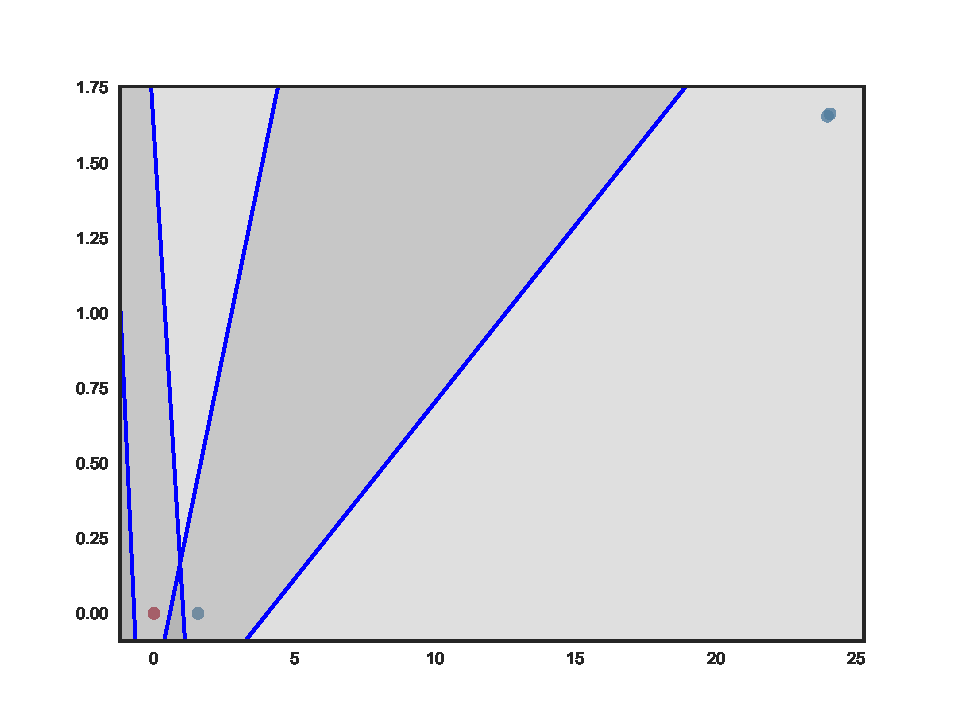
\includegraphics[width=\hsize]{img/toy/unitpointwise/conv2d_25-0.pdf}}
    %   \vskip1em
      \subcaptionbox{25th layer\label{fig:moonsUnitpointwise252}}{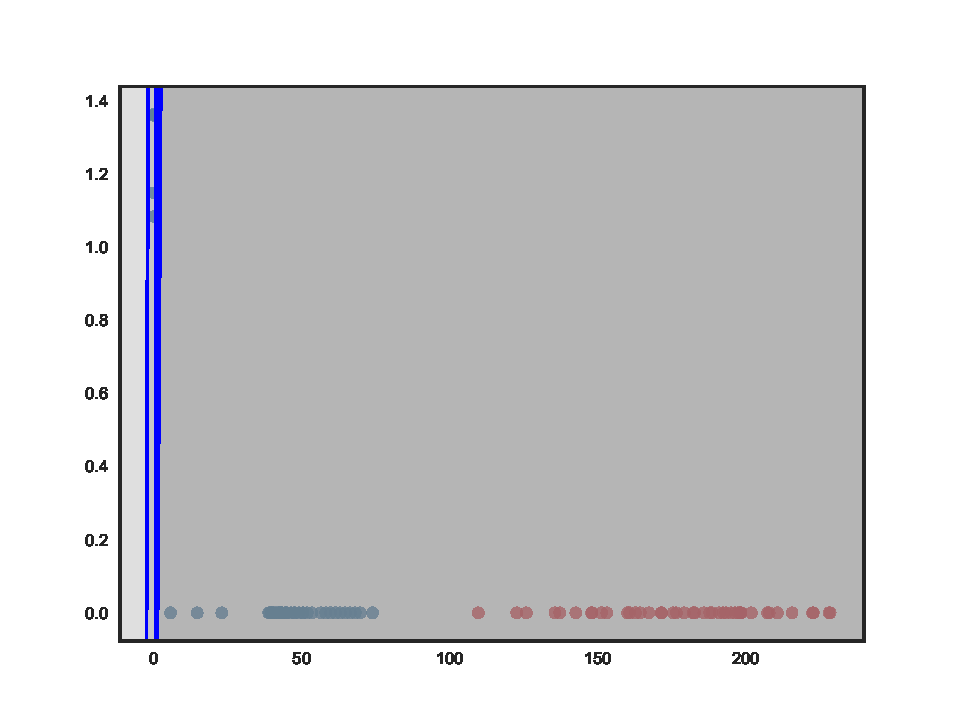
\includegraphics[width=\hsize]{img/toy/unitpointwise/conv2d_25-2.pdf}} 
    }
    % \hskip1em
    \parbox{.195\textwidth}{%
      \subcaptionbox{Feature layer\label{fig:moonsUnitpointwiseFeature1}}{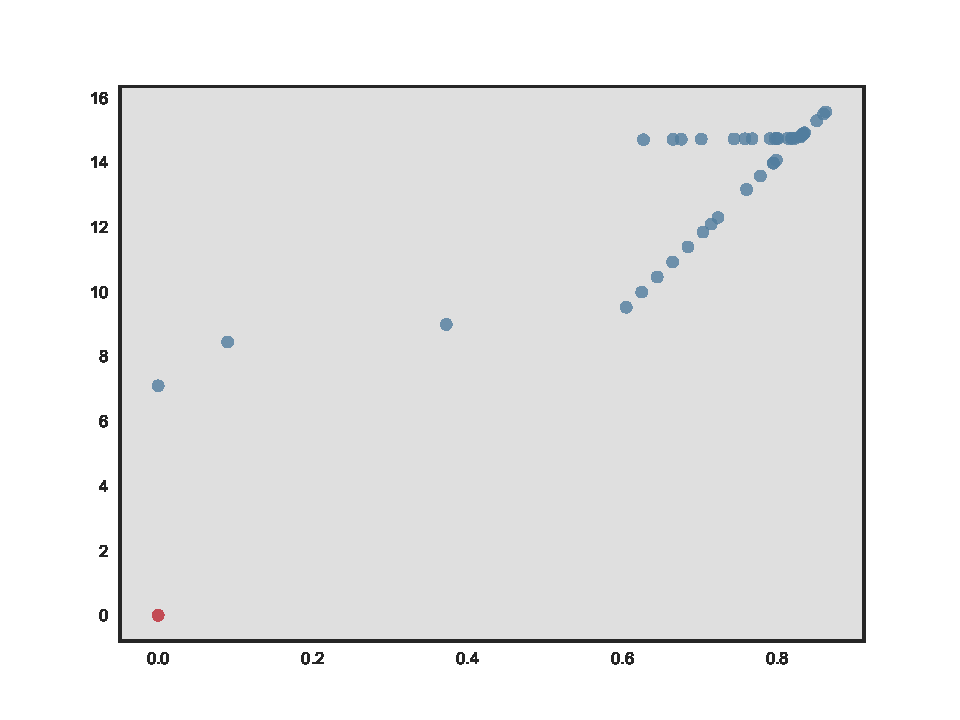
\includegraphics[width=\hsize]{img/toy/unitpointwise/dense_1-0.pdf}}
    %   \vskip1em
      \subcaptionbox{Feature layer\label{fig:moonsUnitpointwiseFeature2}}{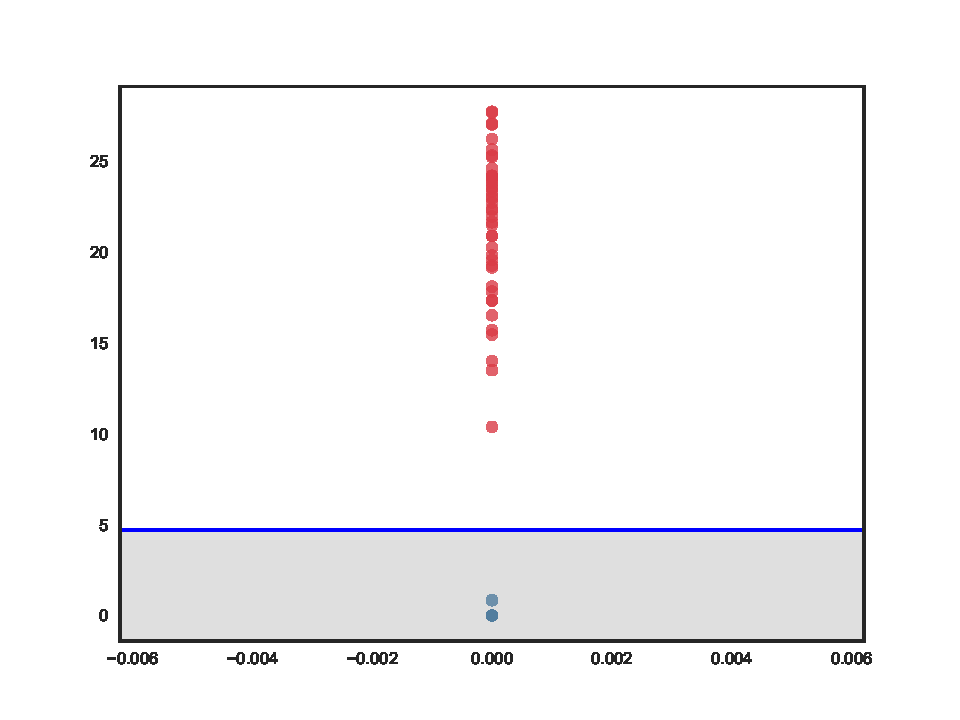
\includegraphics[width=\hsize]{img/toy/unitpointwise/dense_1-2.pdf}} 
    }
    % \hskip1em
    \parbox{.195\textwidth}{%
      \subcaptionbox{Output\label{fig:moonsUnitpointwiseOutput}}{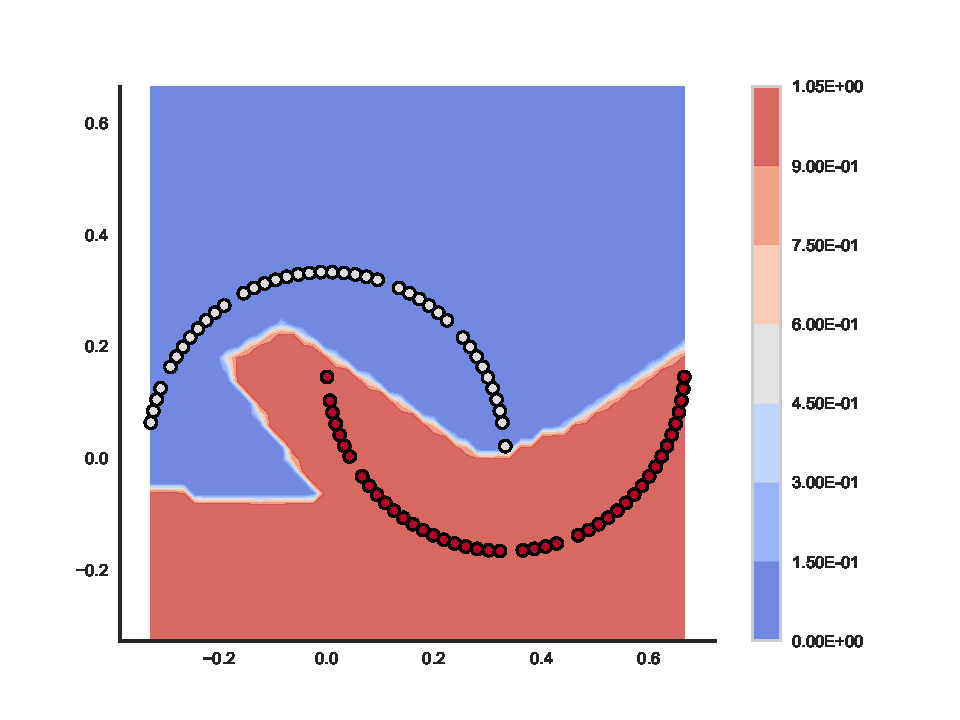
\includegraphics[width=\hsize]{img/toy/unitpointwise/output.pdf}}
    }
  }

    \caption{\SepUnitPoint}
    \label{fig:moonsUnitpointwise}
\end{figure*}

Finally, combining \SepUnit with \SepPoint in \SepUnitPoint effectively separates the classes at Figure \ref{fig:moonsUnitpointwise} (h). The solution found is a bit different from \SepLayer at Figure \ref{fig:moonsLayerwise}(h). We argue that this is due the increased non-linearity of \SepUnit over \SepLayer.

\subsection{The Effect of Constraint Loss}\label{subsec:effectConstraintLoss}

One interesting matter is to understand which effect has the separation constraint by itself, without loss functional. Therefore, we train the same network and hyperparameters than the previous experiment  \ref{subsec:classification}. Then we optimize only the constraints without any other loss. We use \ReLU and \ReLUBN for comparison purposes. 

We find that both \ReLU and \ReLUBN tend concentrate all the data whereas \SepUnitPoint and \SepLayer are able to preserve topological structure, see figure \ref{fig:init}. This explains the failure in \ref{fig:moonsReLU} and \ref{fig:moonsReLUBN}. 
In the other hand, we find how \SepLayer connects the output with in the input by sort of linearizing the network in figures \ref{fig:layerwiseInit501} and \ref{fig:layerwiseInit501}, thus outputting something very similar to a linear classifier. This is consistent with \cite{batchnormGradientExplosion}, where the authors claim that the network performs best as the units work closest to the linear regime. 
\SepUnitPoint output in figures \ref{fig:unitpointInit501} and \ref{fig:unitpointInit502} is less smooth than \SepLayer but still reasonable showing connectivity among the points, proof that topological structure is preserved up to some extent. Notice how the shape of the input layer is quite similar to the final solution found in Figure \ref{fig:moonsUnitpointwise}(a) when using a loss functional, but the feature layer is much more spread. 

We argue that this separation induced by the constraints is responsible of the superior performance shown in \ref{subsec:classification}.

This pursue of separation translates during training into the dynamics shown in figure \ref{fig:peaks}, where we can see the convergence plot for \SepUnitPoint, where the constraint loss and cross-entropy compete each other. The constraint loss pulls the weights into directions which harm cross-entropy thus lowering accuracy, but that are better on the long run, so after fulfilling separation, when cross-entropy converges, the network achieves better accuracy than before the drop. Nevertheless, this behaviour is unstable and sometimes the constraint loss breaks the training process after some iterations.

\begin{figure*}
  \centering
    \begin{subfigure}[b]{0.3\textwidth}
        \includegraphics[width=\textwidth]{img/init/relu/conv2d_1-0.pdf}
        \caption{\ReLU input layer}
        \label{fig:reluInitInput}
    \end{subfigure}
    ~ %add desired spacing between images, e. g. ~, \quad, \qquad, \hfill etc. 
      %(or a blank line to force the subfigure onto a new line)
    \begin{subfigure}[b]{0.3\textwidth}
        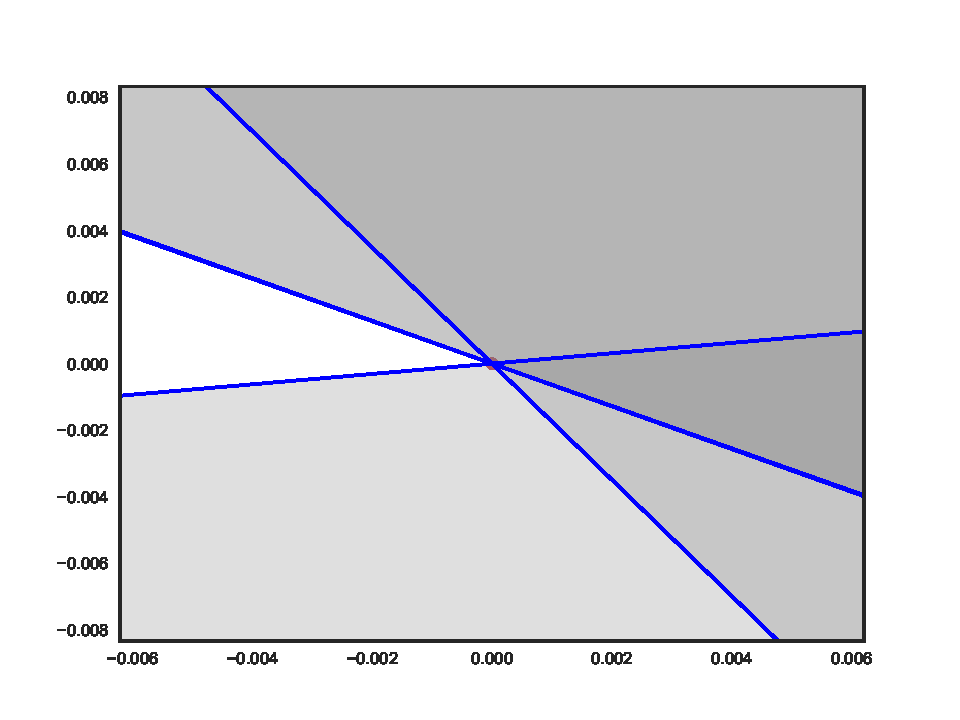
\includegraphics[width=\textwidth]{img/init/relu/conv2d_50-0.pdf}
        \caption{\ReLU 50th layer}
        \label{fig:reluInit501}
    \end{subfigure}
    ~ %add desired spacing between images, e. g. ~, \quad, \qquad, \hfill etc. 
    %(or a blank line to force the subfigure onto a new line)
    \begin{subfigure}[b]{0.3\textwidth}
        \includegraphics[width=\textwidth]{img/init/relu/conv2d_50-2.pdf}
        \caption{\ReLU 50th layer}
        \label{fig:reluIniti502}
    \end{subfigure}
    \\
    \begin{subfigure}[b]{0.3\textwidth}
        \includegraphics[width=\textwidth]{img/init/relu-bn/conv2d_1-0.pdf}
        \caption{\ReLUBN input layer}
        \label{fig:reluBNInitInput}
    \end{subfigure}
    ~ %add desired spacing between images, e. g. ~, \quad, \qquad, \hfill etc. 
      %(or a blank line to force the subfigure onto a new line)
    \begin{subfigure}[b]{0.3\textwidth}
        \includegraphics[width=\textwidth]{img/init/relu-bn/conv2d_50-0.pdf}
        \caption{\ReLUBN 50th layer}
        \label{fig:reluBNInit501}
    \end{subfigure}
    ~ %add desired spacing between images, e. g. ~, \quad, \qquad, \hfill etc. 
    %(or a blank line to force the subfigure onto a new line)
    \begin{subfigure}[b]{0.3\textwidth}
        \includegraphics[width=\textwidth]{img/init/relu-bn/conv2d_50-2.pdf}
        \caption{\ReLUBN 50th layer}
        \label{fig:reluBNInit502}
    \end{subfigure}
    \\
    \begin{subfigure}[b]{0.3\textwidth}
        \includegraphics[width=\textwidth]{img/init/layerwise/conv2d_1-0.pdf}
        \caption{\SepLayer input layer}
        \label{fig:layerwiseInitInput}
    \end{subfigure}
    ~ %add desired spacing between images, e. g. ~, \quad, \qquad, \hfill etc. 
      %(or a blank line to force the subfigure onto a new line)
    \begin{subfigure}[b]{0.3\textwidth}
        \includegraphics[width=\textwidth]{img/init/layerwise/conv2d_50-0.pdf}
        \caption{\SepLayer 50th layer}
        \label{fig:layerwiseInit501}
    \end{subfigure}
    ~ %add desired spacing between images, e. g. ~, \quad, \qquad, \hfill etc. 
    %(or a blank line to force the subfigure onto a new line)
    \begin{subfigure}[b]{0.3\textwidth}
        \includegraphics[width=\textwidth]{img/init/layerwise/conv2d_50-2.pdf}
        \caption{\SepLayer 50th layer}
        \label{fig:layerwiseInit502}
    \end{subfigure}
    \\
    \begin{subfigure}[b]{0.3\textwidth}
        \includegraphics[width=\textwidth]{img/init/unitpointwise/conv2d_1-0.pdf}
        \caption{\SepUnitPoint Input}
        \label{fig:unitpointInitInput}
    \end{subfigure}
    ~ %add desired spacing between images, e. g. ~, \quad, \qquad, \hfill etc. 
      %(or a blank line to force the subfigure onto a new line)
    \begin{subfigure}[b]{0.3\textwidth}
        \includegraphics[width=\textwidth]{img/init/unitpointwise/conv2d_50-0.pdf}
        \caption{\SepUnitPoint 50th layer}
        \label{fig:unitpointInit501}
    \end{subfigure}
    ~ %add desired spacing between images, e. g. ~, \quad, \qquad, \hfill etc. 
    %(or a blank line to force the subfigure onto a new line)
    \begin{subfigure}[b]{0.3\textwidth}
        \includegraphics[width=\textwidth]{img/init/unitpointwise/conv2d_50-2.pdf}
        \caption{\SepUnitPoint 50th layer}
        \label{fig:unitpointInit502}
    \end{subfigure}
    
  \caption{} 
  \label{fig:init} 
\end{figure*}





\begin{figure*}[h]
  \begin{center}
    \includegraphics[width=1.0\textwidth]{peaks}
      \caption{Evolution of training throughout epochs (cross-entropy, constraint loss, and accuracy). Left-hand axis show the accuracy metric (blue line) against the cross-entropy, and constraint loss in the right axis (orange line), for each epoch of the training phase in the horizontal axis.}
			\label{fig:peaks}
\end{center}
\end{figure*}





\subsubsection{Zero initialization}\label{subsec:zero}

We set the parameters to zero in an attempt to simplify initialization. We leave the responsibility of pulling the parameters from zero to the constraint, taking advantage of the fact of that the constraint gradient depend on the input of the units. However, we have two problems: (1) all the units in the layer will share the same gradient and will became the same and, (2) During the first iterations $\xi^+ = \xi^-$, so the gradient from the positive constraint will cancel with the negative.
In order to \emph{break symmetry} of the layers, we use Dropout \cite{dropout}. We find that Dropout has a very strong effect, harming convergence. This is why we choose to use Annealed Dropout \cite{dropoutAnnealing}, starting with a rate of 0.5 for 500 epochs with linear decay. We address the positive and negative constraints cancelling each other by introducing a variable to balance them, see \ref{eq:definitionOfRho}. 
See Figure \ref{fig:zeros} to see how the network evolves until finds a solution. We would like to remark that in this setup the training dynamics become particularly wild in a fashion similar to \ref{fig:peaks}, with several peaks in the constraint loss which ultimately lead to the readjustment of the planes so a solution can be found. Also, we find this process depends on the position of the hyperplanes set during the dropout annealing, introducing an stochastic behaviour that we would prefer to avoid. Finding another mechanism to \emph{break symmetry} would be interesing.



\begin{figure*}
  \centering
    \begin{subfigure}[b]{0.5\textwidth}
        \includegraphics[width=\textwidth]{img/zero/3000/09-conv2d_1-0.pdf}
        \caption{Input layer}
        \label{fig:zerosInput3000}
    \end{subfigure}
    ~ %add desired spacing between images, e. g. ~, \quad, \qquad, \hfill etc. 
      %(or a blank line to force the subfigure onto a new line)
    \begin{subfigure}[b]{0.5\textwidth}
        \includegraphics[width=\textwidth]{img/zero/3000/57-09-output.pdf}
        \caption{Output layer}
        \label{fig:zerosOutput3000}
    \end{subfigure}
    
      
  \caption{Zero initialization plus \SepUnitPoint and annealed dropout} 
  \label{fig:zeros} 
\end{figure*}


\subsection{Results concerning Accuracy}\label{subsec:accuracyResults}

To gauge accuracy between \ReLU, \ReLU +  batchnorm (\ReLUBN), and our proposal we tested all variants of our constraint using the same setup as \ref{subsec:classification}. We sampled $100$ points ($85$ for training and $15$). We used a 50x4 network. As hyper-parameters, we used learning rates $\gamma \in \{0.01, 0.001, 0.0001\}$, a batch size $bs = 85$, constraint loss parameter $\lambda = 0.01$ when needed, and set the number of epochs to $T = 2000$. We used the Glorot initialization scheme \cite{Glorot10Initialization}. 
 
We find how any of \SepConstraint versions show significant improvements over the \ReLU and \ReLUBN baselines (which yield \emph{trivial} validation accuracies of $40$\% and $60$\%, respectively). In the other hand, we see how \SepLayer achieves perfect accuracy closely followed by \SepUnitPoint, whereas \SepUnit and \SepPoint lag a bit behind, mirroring the results from \ref{subsec:classification}. The reader can observe Table \ref{tab:moons} for further detail.


\begin{table}[h!]
\begin{center}
\begin{tabular}{l|rr|rr}
\toprule
{}  & \multicolumn{2}{c}{Accuracy} & \multicolumn{2}{c}{Loss} \\
{}  & Train   & Val.  & Train  & Val.  \\
\midrule
\ReLU            &  0.5176 &      0.4 &  0.6925 &  0.6938 \\
\ReLUBN     &  0.8117 &      0.6 &  0.6331 &  0.6636 \\
\SepLayer &  1.0000 &      1.0 &  0.0000 &  0.0211 \\
\SepPoint    &  0.9294 &  0.8000 &  0.1765 &  0.6476 \\
\SepUnit    &  0.9058 &  0.8000 &  0.4161 &  1.5228 \\
\SepUnitPoint   &  0.9882 &  0.9333 &  0.6988 &  1.0810 \\
\bottomrule
\end{tabular}
\end{center}
\caption{Maximal performance experiment using the \moons dataset. From left to right, accuracy and loss (for \emph{train} and \emph{validation} sets) for \ReLU, \ReLUBN, and  \SepConstraint in all its variants.}
  \label{tab:moons}
\end{table}

